\documentclass{beamer} %
\usetheme{Montpellier}       % or try default, 
%  \setbeamertemplate{navigation symbols}{}
%\usetheme[compressed]{Singapore}
\useinnertheme{circles}
%\useoutertheme{miniframes}
\setbeamertemplate{caption}[numbered]
\setbeamersize{text margin left=5mm,text margin right=10mm}
\usepackage[latin1]{inputenc}
%\usefonttheme{serif}
%\usepackage{times}
%\usepackage{palatino}
\usepackage{tikz}
\usepackage{dcolumn}
\usepackage{amsmath}
\usepackage{verbatim}
\usepackage{booktabs}
\usepackage{color, colortbl} %righe colorate
\usetikzlibrary{mindmap,calc,patterns,decorations.pathmorphing,decorations.markings, arrows, shapes.arrows, shapes, backgrounds, positioning}
%\usetikzlibrary{arrows,shapes}
\usepackage[absolute,overlay]{textpos}
\usepackage{spot}
\usepackage{graphicx}
\usepackage{subcaption}
\usepackage{lmodern}
\usepackage[scale=2]{ccicons}
\usepackage{xcolor}
\usepackage{multirow}
\usepackage{animate}
\usepackage{listings}
\usepackage{amsmath}
\usepackage[flushleft]{threeparttable}
\usepackage{picture}
\usepackage[letterspace=150]{microtype}
\usepackage[absolute,overlay]{textpos}
\usepackage{tikzsymbols}
\usepackage{setspace}
\let\svthefootnote\thefootnote
\usepackage{animate}
\usepackage{xmpmulti}
\usepackage{tabularx}
\usepackage{array}
\usepackage{bm}
\usetikzlibrary{matrix}
\usepackage{color, colortbl} %righe colorate
\newcolumntype{d}[1]{D{.}{.}{#1}}

\DeclareMathOperator*{\argmax}{arg\,max}
\newcolumntype{P}[1]{>{\centering\arraybackslash}p{#1}}
\textheight 1in
\newcommand\Factor{1.2}
\setbeamersize{text margin left=5mm,text margin right=10mm}
\setbeamerfont{subtitle}{size=\large, series=\bfseries}
%\definecolor{template}{RGB}{54, 114, 89}
%\definecolor{template}{RGB}{181, 18, 27}
\definecolor{template}{RGB}{70, 130, 180}
% Per il tema Montpellier
\setbeamercolor{separation line}{bg=template}
\setbeamercolor{title in head/foot}{bg=background, fg=template}
\setbeamercolor{section in head/foot}{bg=background, fg=template}
\setbeamercolor{subsection in head/foot}{bg=background, fg=template}
\setbeamercolor{background canvas}{bg=background}
\setbeamercolor{section in toc}{fg=template}
\setbeamercolor{subsection in toc}{fg=black}
\setbeamerfont{section in toc}{series=\bfseries,size=\normalsize}
\setbeamerfont{title}{family=\scshape}

% per gli alri temi
%\definecolor{background}{RGB}{250, 250, 250}
\definecolor{background}{RGB}{255, 255, 255}
\setbeamercolor{frametitle}{fg=template, bg=background}
%\setbeamercolor{section in head/foot}{bg=template, fg=template!20}
%\setbeamercolor{subsection in head/foot}{bg=template!20, fg=template}
%\setbeamercolor{author in head/foot}{bg=template, fg=template!20}
%\setbeamercolor{date in head/foot}{bg=template, fg=white}
%\setbeamercolor{page number in head/foot}{bg=template, fg=white}
%\setbeamercolor{title in head/foot}{fg=template}
%\setbeamercolor*{item}{fg=template}
\setbeamertemplate{frametitle}[default][center]
\setbeamercolor{title}{fg=template}
\definecolor{highlight}{RGB}{54, 114, 89}
\definecolor{back}{RGB}{247, 251, 255}
\definecolor{map}{RGB}{111, 172, 232}
\definecolor{childmap}{RGB}{161, 200, 240}
\definecolor{nodemap}{RGB}{141, 170, 199}
\definecolor{rasch}{rgb}{0.0, 0.33, 0.71}
\definecolor{log}{rgb}{0.0, 0.65, 0.58}
\definecolor{diff}{RGB}{33, 113, 181}
\definecolor{single}{RGB}{106, 81, 163}
\definecolor{comp}{RGB}{35, 99, 70}
\definecolor{inc}{RGB}{191, 13, 43}
\definecolor{highlight}{rgb}{0.45, 0.31, 0.59}
\definecolor{section}{RGB}{51,51,179}
\definecolor{typical}{RGB}{8, 69, 148}
\definecolor{model}{RGB}{74, 20, 134}
\definecolor{orangered2}{RGB}{238,64,0}
\definecolor{royalblue3}{RGB}{58,95,205}
\definecolor{springgreen}{RGB}{0,205,102}
\definecolor{magenta}{RGB}{255,0,255}
\definecolor{seagreen}{RGB}{75, 155, 110}
\definecolor{bp}{RGB}{248,114,105}
\definecolor{uip}{RGB}{199,124,255}
\definecolor{eip}{RGB}{121,172,0}
\definecolor{rp}{RGB}{0,187,192}


%\setbeamertemplate{frametitle}[default][center]

\setbeamerfont{frametitle}{size=\large, series=\bfseries, family=\scshape}
\setbeamerfont{subtitle}{size=\large, series=\bfseries}


\DeclareMathOperator*{\E}{\mathbb{E}}

%\linespread{1.2}\selectfont 

  \tikzset{
	invisible/.style={opacity=0},
	visible on/.style={alt={#1{}{invisible}}},
	alt/.code args={<#1>#2#3}{%
		\alt<#1>{\pgfkeysalso{#2}}{\pgfkeysalso{#3}} % \pgfkeysalso doesn't change the path
	},
	every overlay node/.style={
		%draw=black,fill=white,rounded corners,
		anchor=north west, inner sep=0pt,
	},
}

\def\tikzoverlay{%
	\tikz[remember picture, overlay]\node[every overlay node]
}%


\newcommand{\tstar}[5]{% inner radius, outer radius, tips, rot angle, options
	\pgfmathsetmacro{\starangle}{360/#3}
	\draw[#5] (#4:#1)
	\foreach \x in {1,...,#3}
	{ -- (#4+\x*\starangle-\starangle/2:#2) -- (#4+\x*\starangle:#1)
	}
	-- cycle;
}

\newcommand{\ngram}[4]{% outer radius, tips, rot angle, options
	\pgfmathsetmacro{\starangle}{360/#2}
	\pgfmathsetmacro{\innerradius}{#1*sin(90-\starangle)/sin(90+\starangle/2)}
	\tstar{\innerradius}{#1}{#2}{#3}{#4}
}

%colonne colorate nelle matrici 

\newcommand{\DoTikzmark}[1]{%
	\tikz[remember picture] \coordinate[shift={(0,.7ex)}](#1);%
}
\newcommand{\colrow}[3][]{%
	\tikz[overlay,remember picture, line width=10pt]
	\draw[shorten >=-.1em, shorten <=-.1em, #1] (#2)--(#3);
}

\AtBeginSection[]
{
	\begin{frame}
		\tableofcontents[currentsection,currentsubsection]
	\end{frame}
}  
\AtBeginSubsection[]
{
	\begin{frame}
		\tableofcontents[currentsection,currentsubsection]
	\end{frame}
}  

\title[Don't say CAT]{Don't say CAT: \\ New Item Response Theory approaches for developing short test forms}
\date[AIP 2022]{XXX Annual Conference of the Italian Psychology Association (AIP)}
\vspace{5mm}
\titlegraphic{%
	
\includegraphics[width=1.8cm,height=1.8cm,keepaspectratio]{img/unipd.png}%\hspace*{9.75cm}~%
	
\includegraphics[width=2.5cm,height=2.5cm,keepaspectratio]{img/psicostat.png}%
	
\includegraphics[width=1.8cm,height=1.8cm,keepaspectratio]{img/unicatt.png}%
}
\institute[]{September 30\textsuperscript{th} 2022, Padova}
\author[O.M.E., P.A., E.R.]{\texorpdfstring{Ottavia M. Epifania\textsuperscript{1,2}, Pasquale Anselmi\textsuperscript{1}, Egidio Robusto\textsuperscript{1}\newline\url{ottavia.epifania@unipd.it} \newline \textsuperscript{1}Univerisity of  Padova\newline\textsuperscript{2}Catholic University of the Sacred Heart}{Author}}

\newcommand\high{\cellcolor{template!20}}

\begin{document}

	
\begin{frame}[plain]
	\maketitle
\end{frame}

\section[Intro]{Introduction}


\begin{frame}{CAT}

	\centering
\begin{overprint}

	\onslide<1>
		\centering
	\begin{tikzpicture}
		\node (img) {
\includegraphics[width =.50\linewidth]{img/cat}};
	\end{tikzpicture}
\onslide<2>
	\centering
\begin{tikzpicture}
	\node (img) {
\includegraphics[width =.50\linewidth]{img/cat}};
	\draw[red, line width=3.4mm] 
	(img.south west) -- (img.north east)
	(img.south east) -- (img.north west);
\end{tikzpicture}

\textcolor{template}{\textbf{C}}omputerized \textcolor{template}{\textbf{A}}daptive \textcolor{template}{\textbf{T}}esting
\end{overprint}


\end{frame}

\begin{frame}{Item Response Theory and short test forms}

\textsc{\textcolor{template}{Adaptive short forms}}: \emph{Ad-hoc} tests for each person \textcolor{template}{$\rightarrow$} The information is maximized for each level of $\theta$ (i.e., for each respondent) \textcolor{template}{$\rightarrow$} (\textcolor{template}{\textbf{CAT}}: Computerized Adaptive Testing)
		
		\onslide<2->
		\begin{alertblock}{Issue}
			
		Different short test forms for each respondent $\rightarrow$ Potential fairness issues in assessments, e.g. for recruitment
		\end{alertblock}
		
		\onslide<1->
\textcolor{template}{\textsc{Static short forms}}: Static tests equal for all respondents \textcolor{template}{$\rightarrow$} The information is maximized across $\theta$ levels (i.e., across all respondents)
		
		\onslide<3->
		\begin{alertblock}{Issue}
		
		Not being tailored to any $\theta$ level of interest \textcolor{template}{$\rightarrow$} Potentially more items are needed to  cover a wide range of $\theta$s
		\end{alertblock}


\end{frame}

\begin{frame}{Aim}
	\tikzoverlay (n1) at (0.2cm,1.3cm) {%
		\begin{minipage}{\textwidth}%
			\begin{block}{}%
				\centering{\large{New IRT-based procedures for shortening tests}}
				
				\vspace{3mm}
				
			\end{block}
		\end{minipage}
	};%
	\onslide<2->
	\tikzoverlay (n2) at (-1cm,-0.5cm) {%
		\begin{minipage}{0.6\textwidth}%
			\begin{block}{}%
				\centering
				Equal for all respondents 
			\end{block}
		\end{minipage}
	};%
	\onslide<3->
	\tikzoverlay (n3) at (5.6cm,-0.5cm) {%
		\begin{minipage}{0.6\textwidth}%
			\begin{block}{}%
				\centering
				Tailored to specific levels of \\ the latent trait
			\end{block}
		\end{minipage}
	};%
	%
	
	\begin{tikzpicture}[remember picture, overlay]
		\onslide<2->  \path [line width=0.04cm,->,shorten >= +3pt, template] (n1.south) edge (n2.north);
		\onslide<3->  \path [line width=0.04cm,->, shorten >= +3pt, template] (n1.south)  edge (n3.north);
	\end{tikzpicture}
	
\end{frame}

\section[IRT and Information Functions]{Item Response Theory and information functions}

\subsection*{2-PL Model}


\begin{frame}{Item Response Theory}{2-PL Model}

				\begin{equation*}\label{eq:2pl}
				P(x_{pj} = 1|\theta_p, b_j, a_j) = \frac{exp[a_j(\theta_p - b_j)]}{1 + exp[a_j(\theta_p - b_j)]}
			\end{equation*}
		\vspace{3mm}
			where: 
		
			$P(x_{pj} = 1)$: Probability of a correct response to item $j$ by respondent $p$
			
				\vspace{1.5mm}
				
			$\theta_p$: Ability of respondent $p$
			
				\vspace{1.5mm}
			$b_j$: Difficulty of item $j$
			
				\vspace{1.5mm}
			$a_j$: Discrimination of item $j$



\end{frame}

\begin{frame}
	\begin{overprint}
		\onslide<1>
		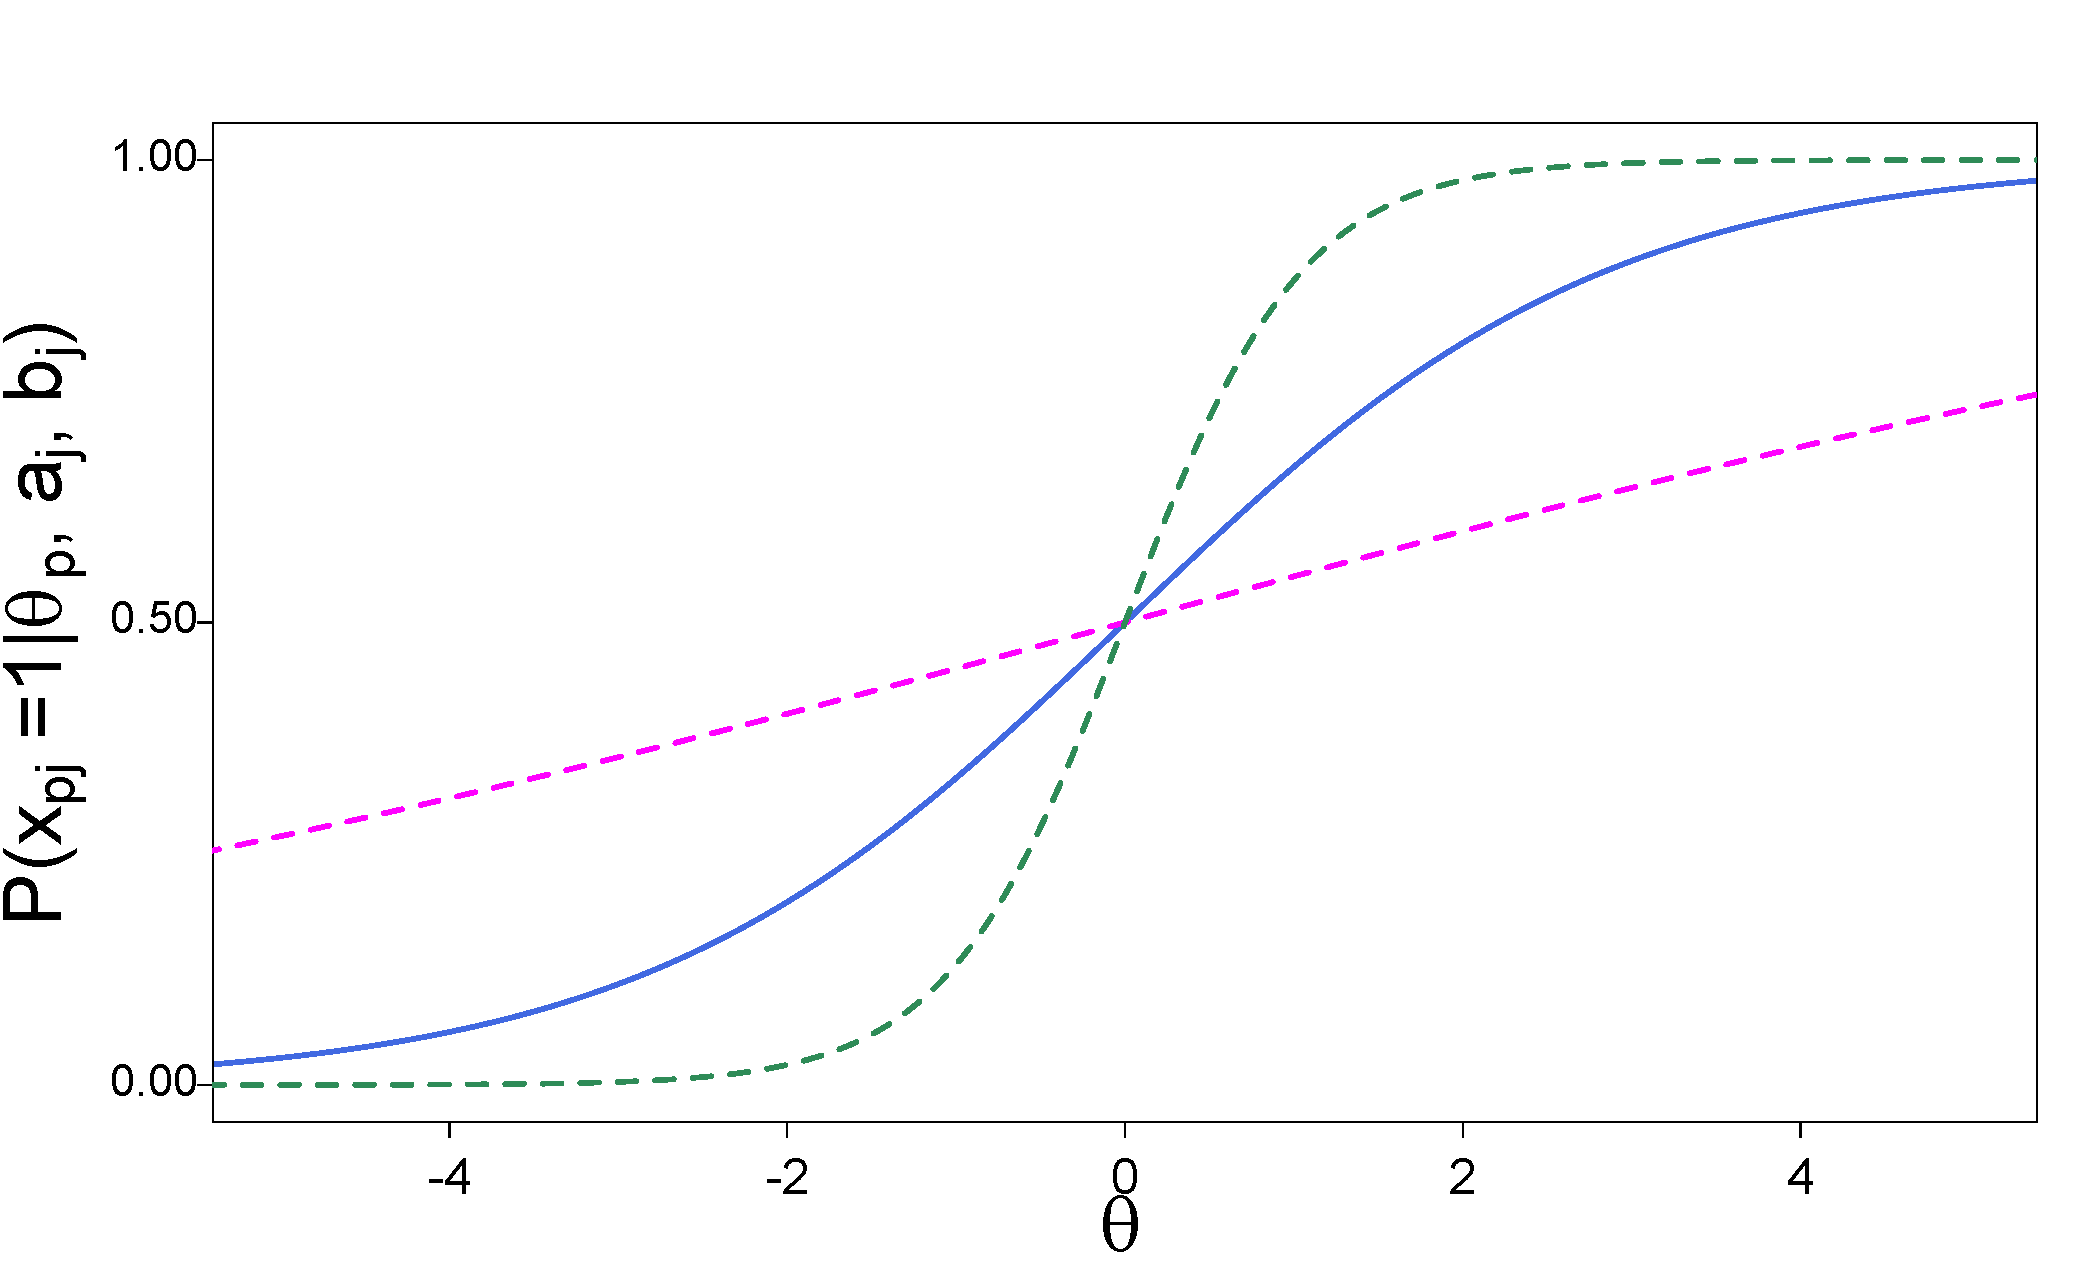
\includegraphics[width=\linewidth]{img/item}
		\onslide<2>
		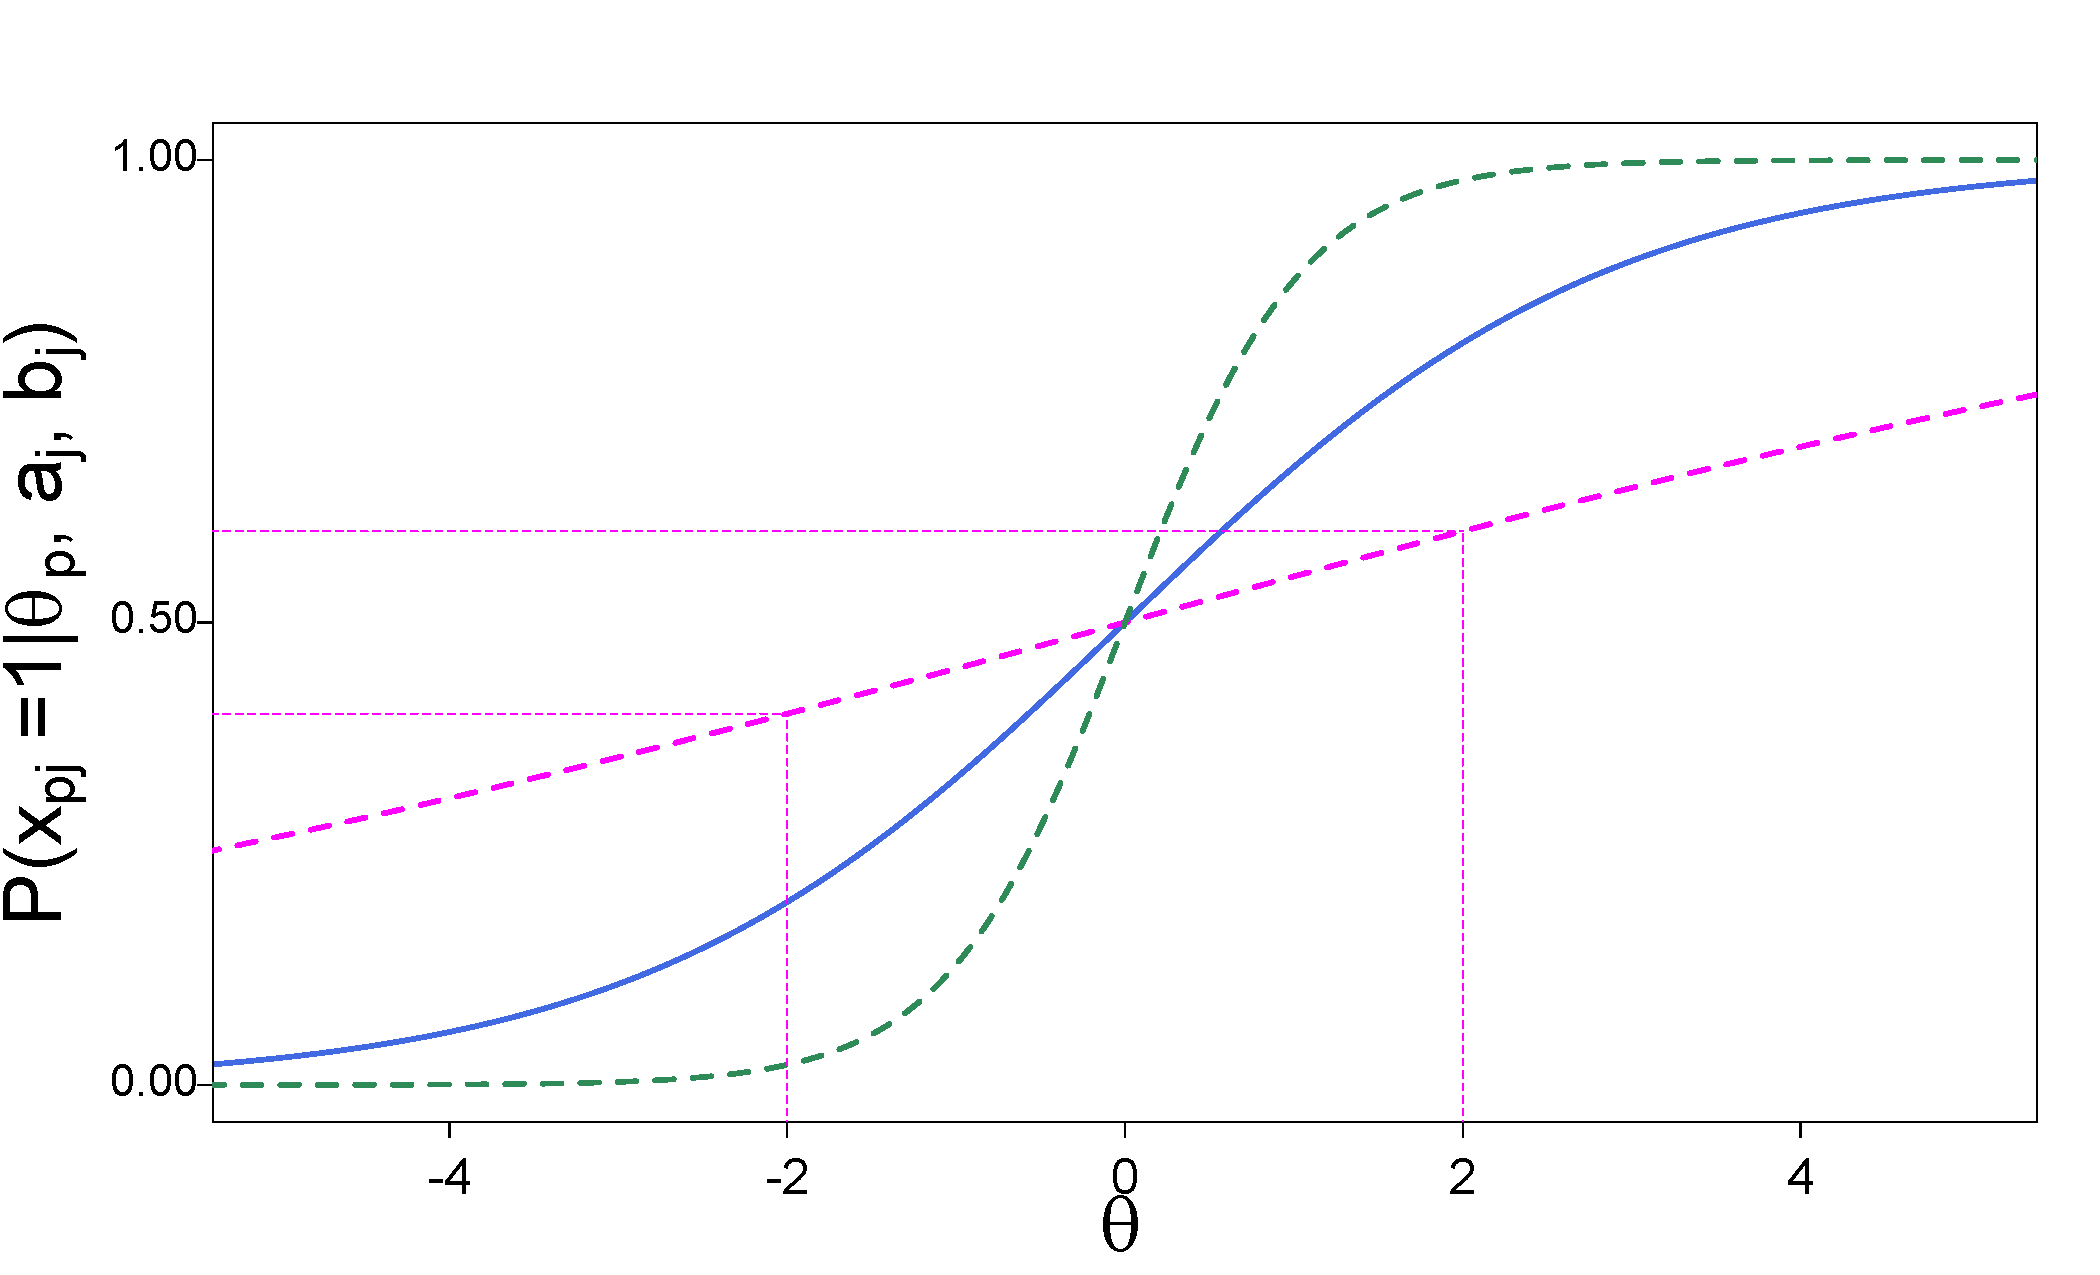
\includegraphics[width=\linewidth]{img/itemA}
		\onslide<3>
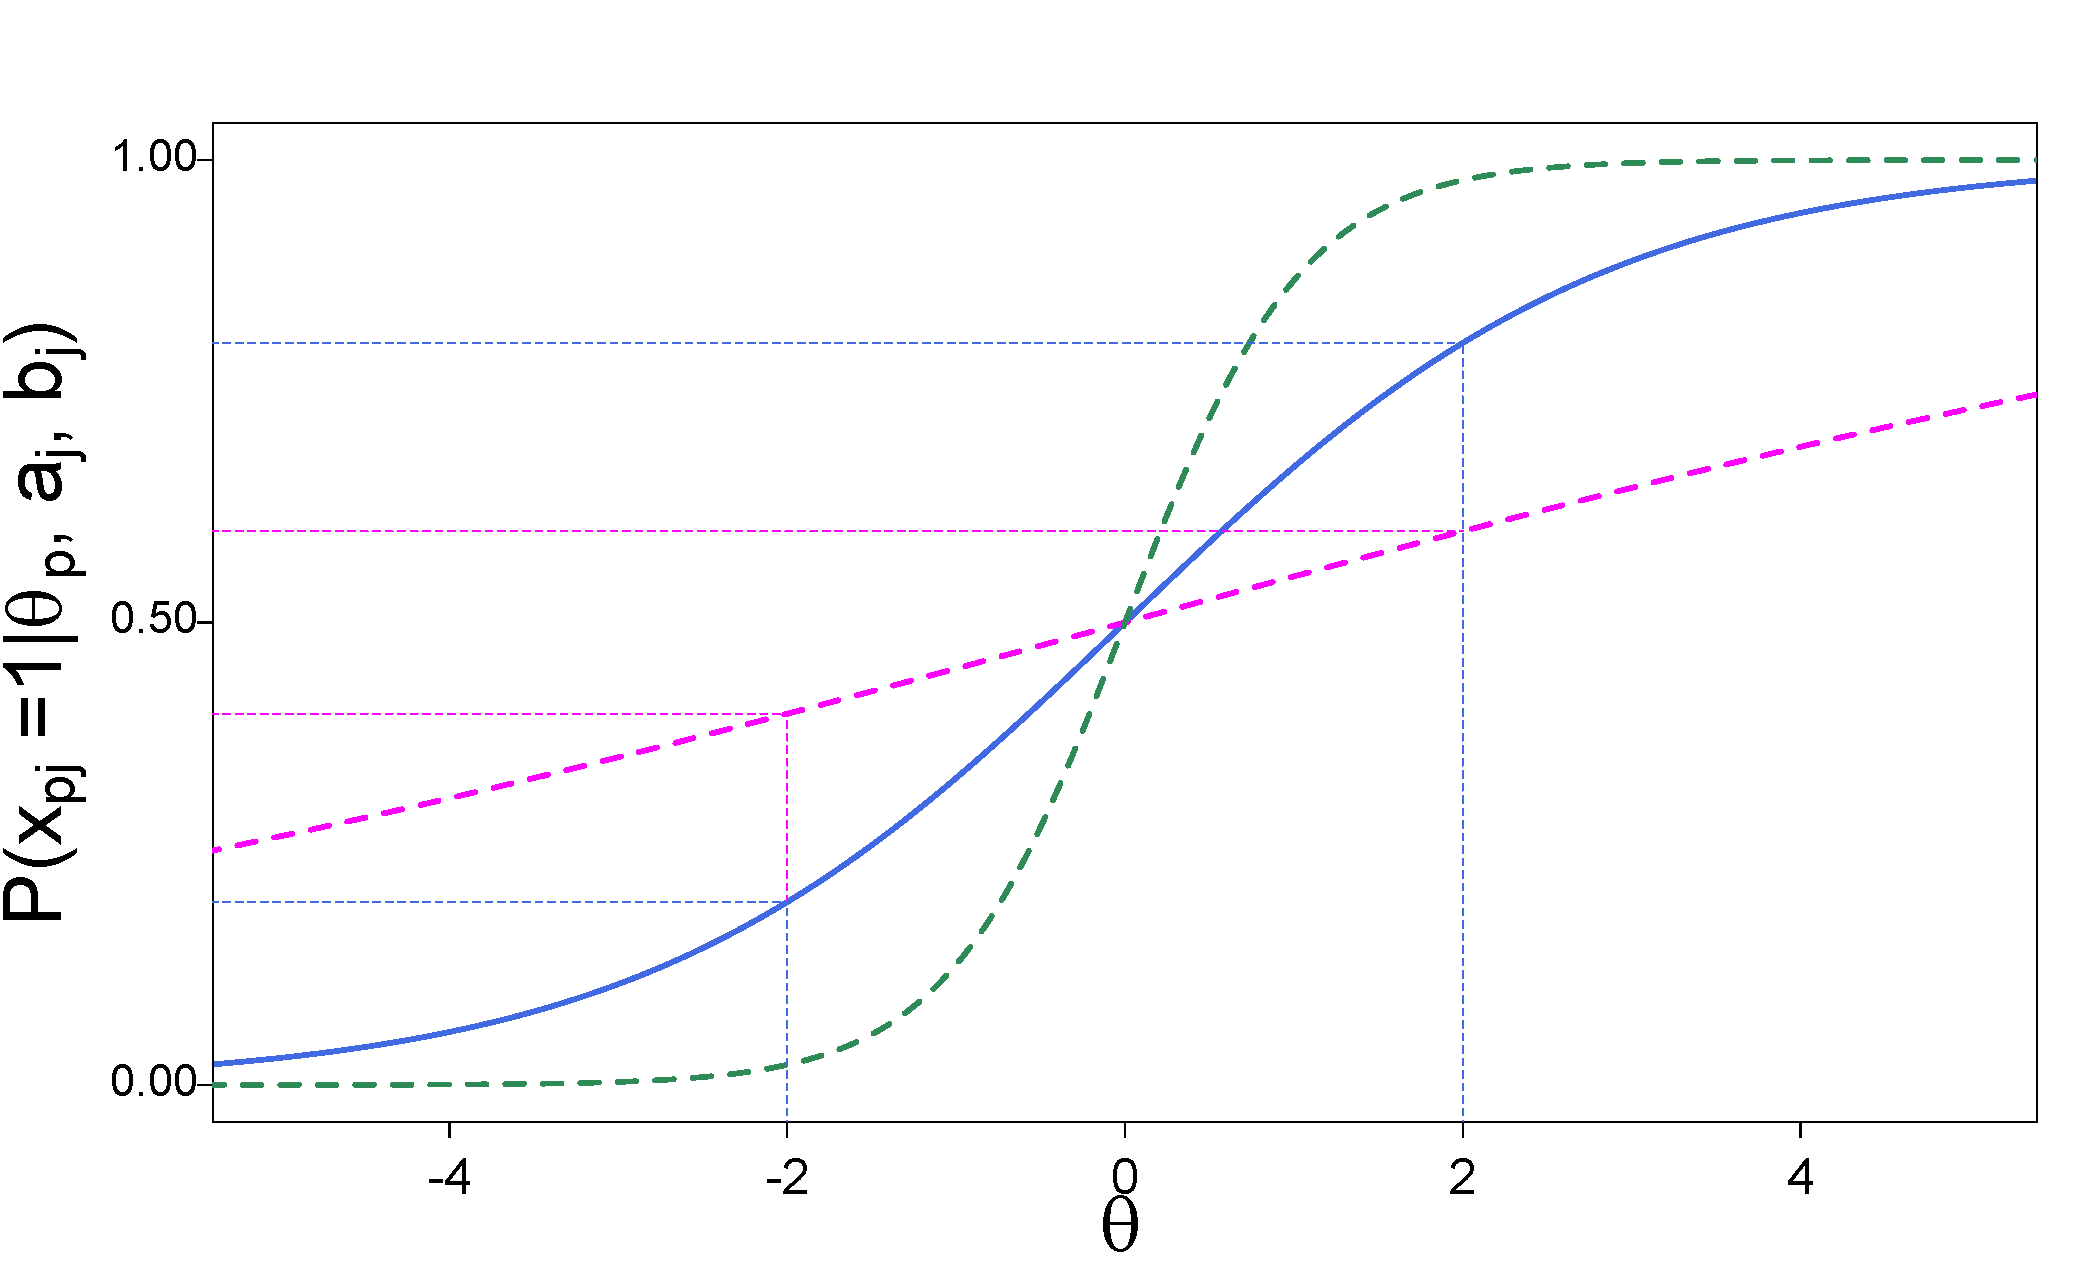
\includegraphics[width=\linewidth]{img/itemB}
\onslide<4>
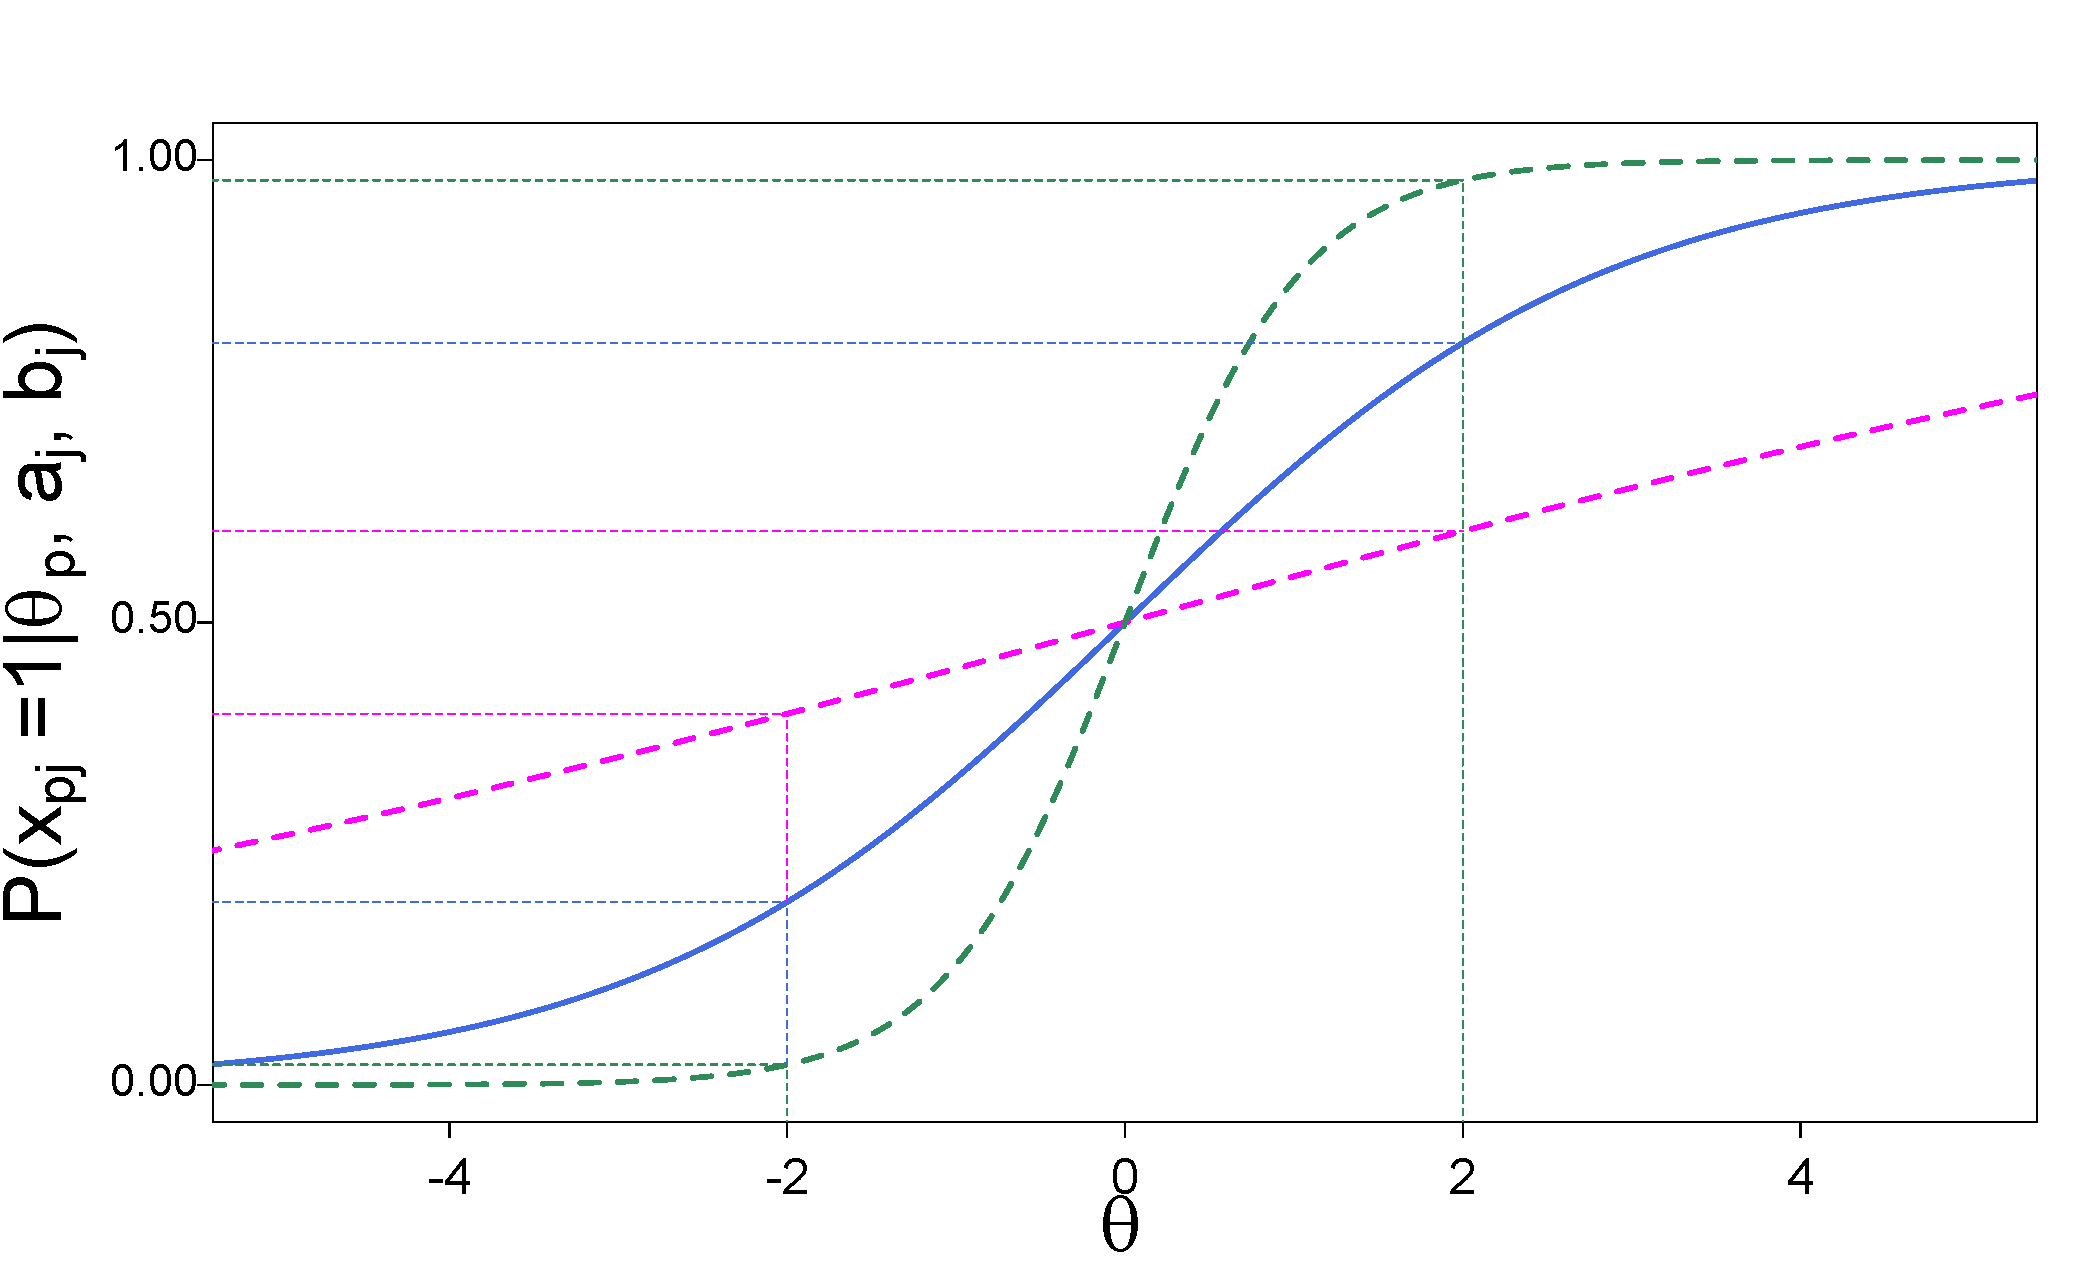
\includegraphics[width=\linewidth]{img/itemC}		
	\end{overprint}
	
\end{frame}

\subsection*{Information functions}
\begin{frame}{Information functions}
	\vspace*{-5mm}
	\begin{columns}[T]
		\begin{column}{.50\linewidth}
				\begin{center}
				Item Information Function
			\end{center}
			\begin{equation*}\label{eq:IIF}
			\mathit{IIF}_j = a_j^2[P(\theta)(1-P(\theta))]
		\end{equation*}
	\pause
	\vspace*{-4mm}
	\begin{figure}
		\centering
			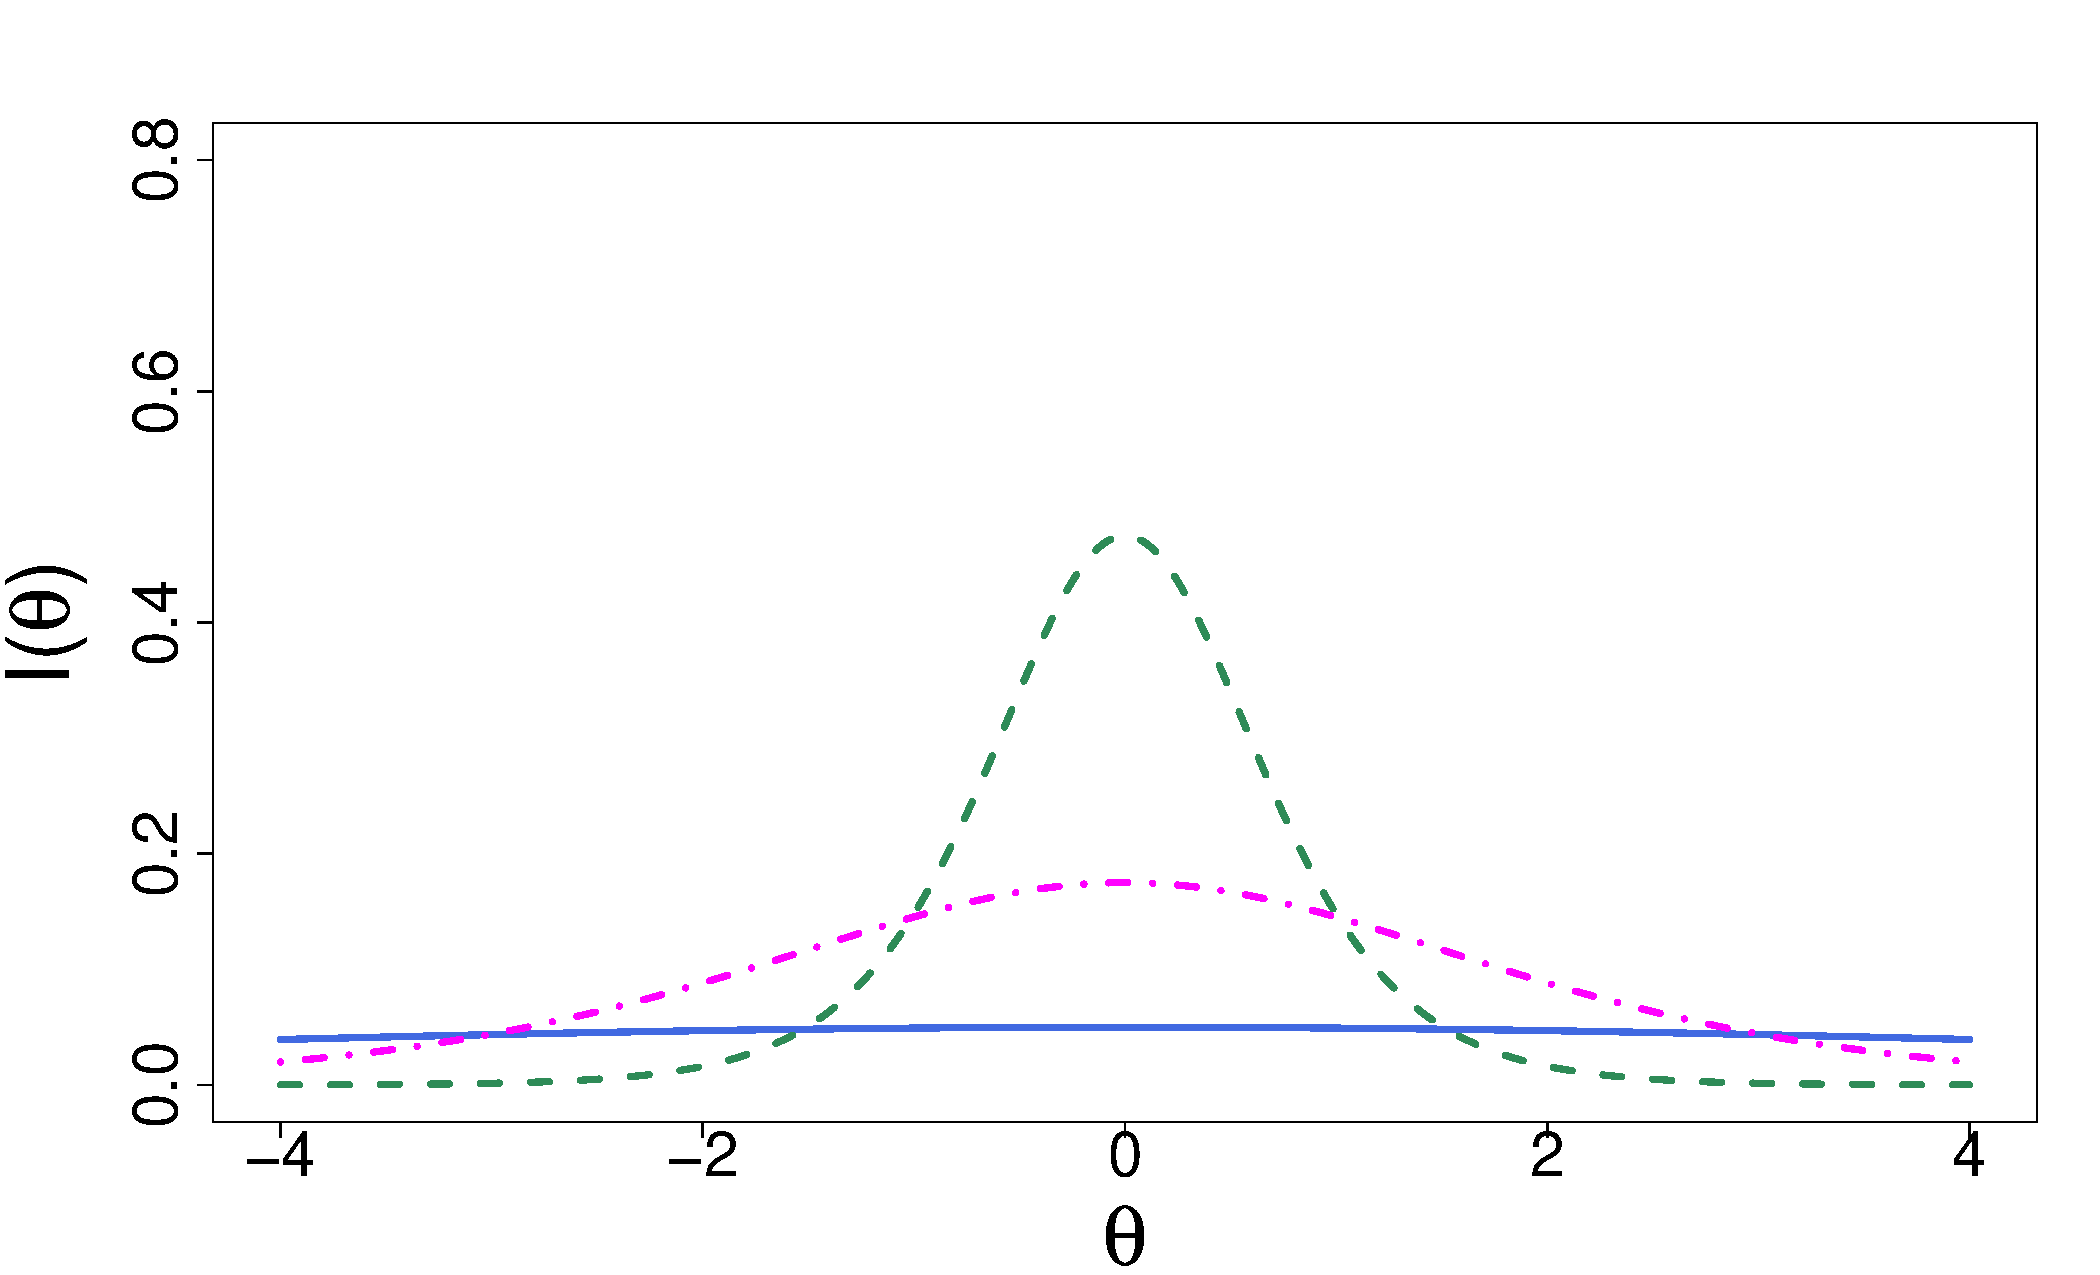
\includegraphics[width=\linewidth]{img/iifs.pdf}
			\caption{\footnotesize{\textcolor{blue}{$a = 0.20$}, \textcolor{magenta}{$a = 0.70$}, 
			\textcolor{seagreen}{$a = 1.90$}, $b=0$}}
\label{sub:iif}
	\end{figure}
		\end{column}
\begin{column}{.50\linewidth}
	\pause
	\begin{center}
		Test Information Function
	\end{center}
	\begin{equation*}\label{eq:TIF}
	\mathit{TIF} = \displaystyle \sum_{j=1}^{J} \mathit{IIF}_j
\end{equation*}
\vspace*{-6mm}
\pause
\begin{figure}
	\centering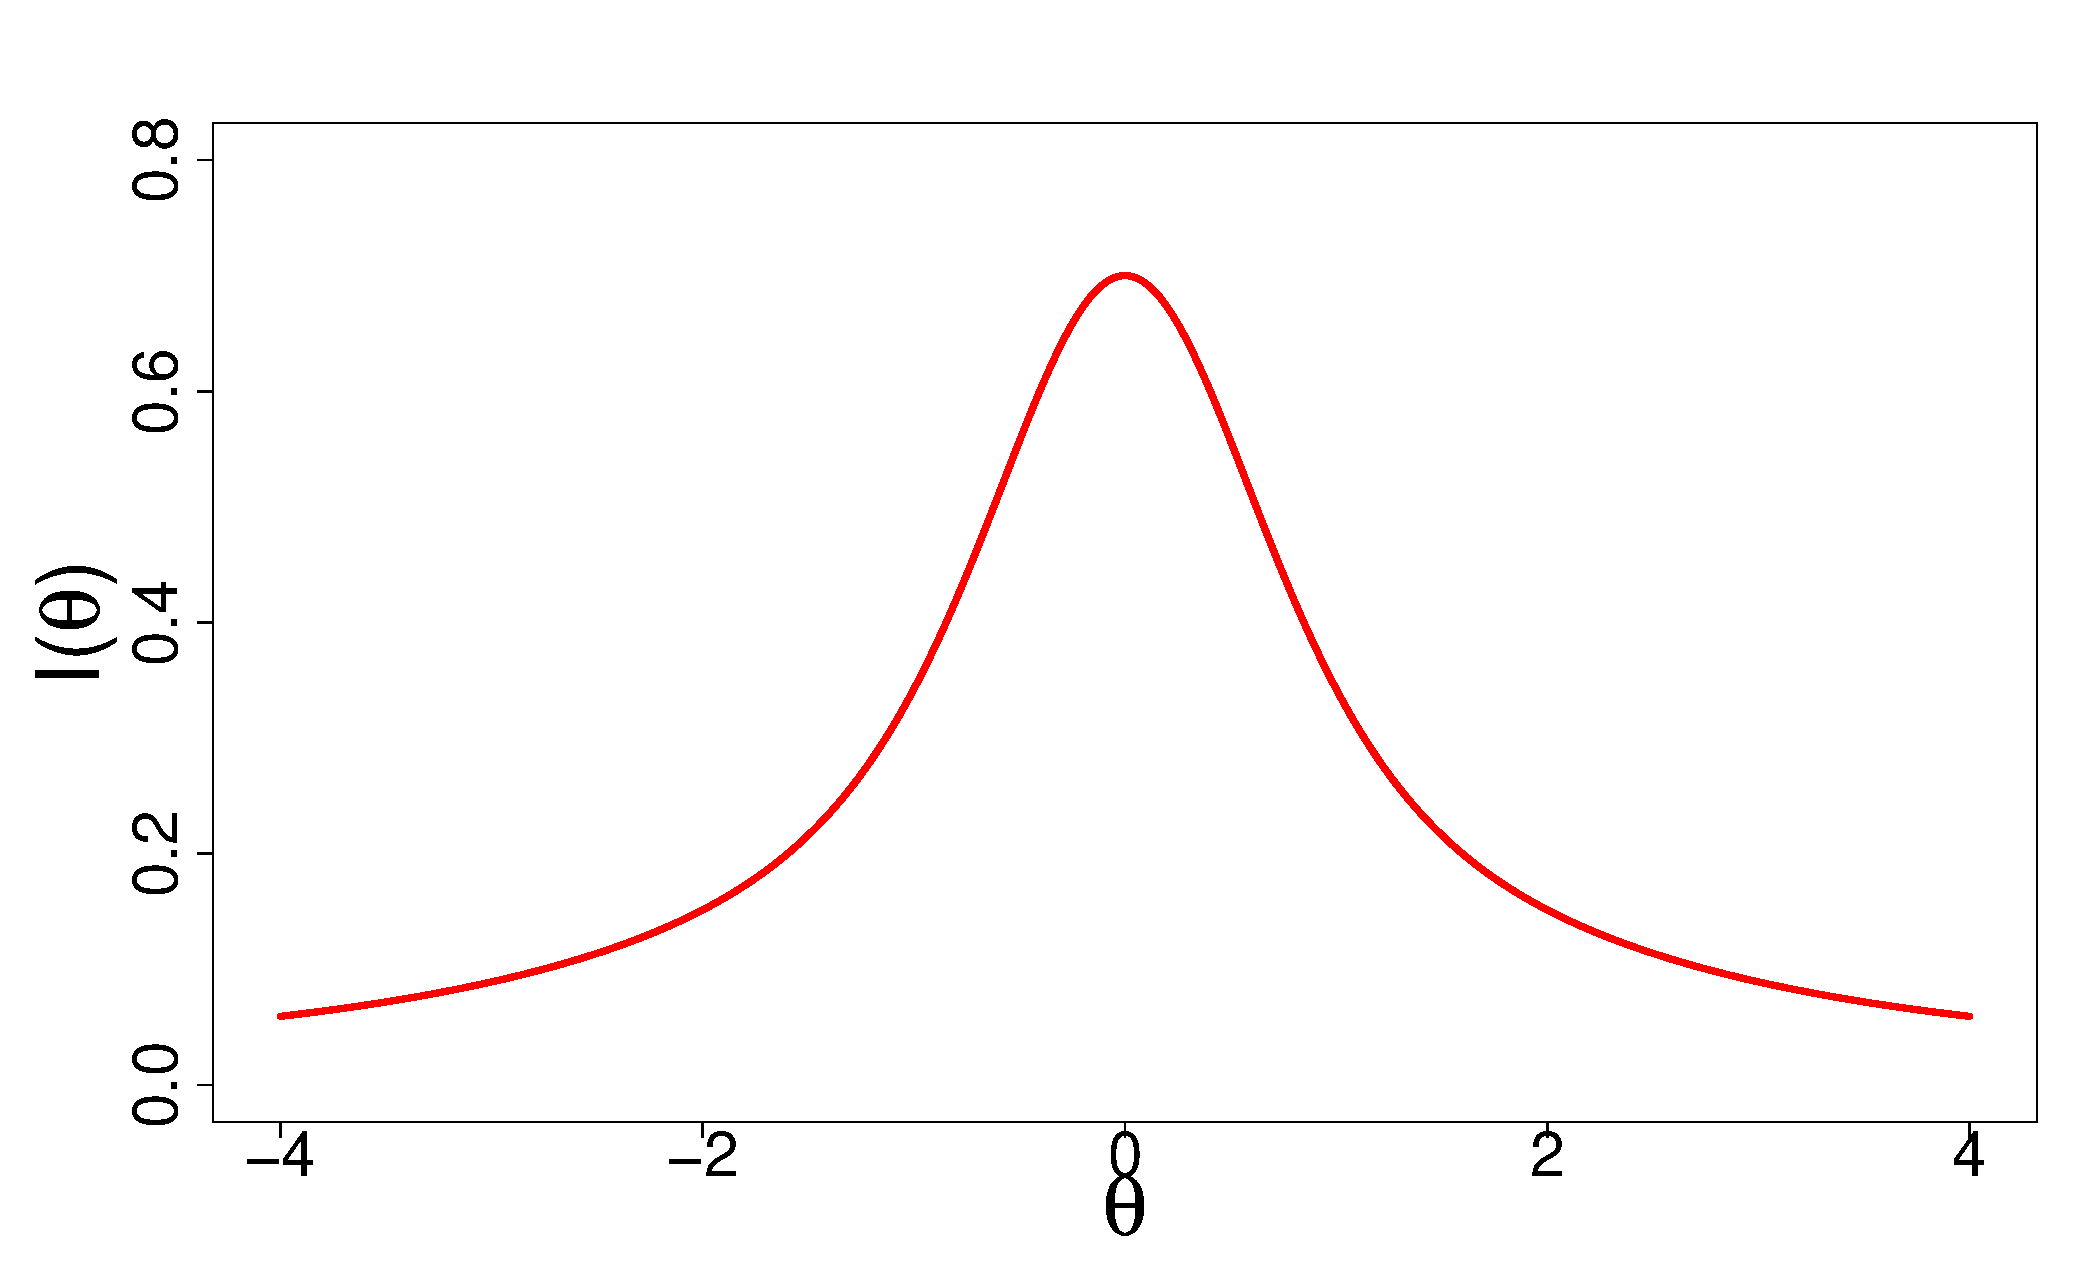
\includegraphics[width=\linewidth]{img/tif.pdf}
	\caption{TIF $=$ \textcolor{blue}{\emph{IIF}$_1$} $+$ \textcolor{magenta}{\emph{IIF}$_2$} $+$ \textcolor{seagreen}{\emph{IIF}$_3$}}
	\label{sub:tif}
\end{figure}

\end{column}
	
\end{columns}
\end{frame}

\section[Short form procedures]{IRT procedures for shortening tests}

\subsection{Benchmark procedure}

\begin{frame}{Benchmark procedure}
	
	Selected items $\rightarrow$ items with the highest \emph{IIF}s 
		
		\vspace{2mm}
		\begin{quote}
		e.g.:	3-item short form from 10-item full-length test
		\end{quote}
	\vspace*{-5mm}
\begin{overprint}
	\onslide<1>
	\vspace{2mm}
	\begin{table}
\begin{tabular}{l  d{3.2}d{3.2}d{3.2}}
	\toprule
	item & b & a & IIF \\
	\midrule
1	& 	-0.67	 & 	0.71	 & 	0.08	\\
2	& 	0.50	 & 	1.19	 & 	0.15	\\
3	& 	-2.43	 & 	0.25	 & 	0.01	\\
4	& 	2.12	 & 	1.98	 & 	0.24	\\
5	& 	1.72	 & 	0.39	 & 	0.03	\\
6	& 	-2.28	 & 	1.62	 & 	0.19	\\
7	& 	0.64	 & 	0.50	 & 	0.05	\\
8	& 	-2.51	 & 	1.68	 & 	0.19	\\
9	& 	-0.66	 & 	0.44	 & 	0.04	\\
10	& 	0.72	 & 	0.33	 & 	0.02	\\
\bottomrule
\end{tabular}
	\end{table}

\onslide<2>
	\vspace{2mm}
	\begin{table}
	\begin{tabular}{l  d{3.2}d{3.2}d{3.2}}
		\toprule
		item & b & a & IIF \\
		\midrule
		\rowcolor{template!20!}4	& 	2.12	 & 	1.98	 & 	0.24	\\
		\rowcolor{template!20!}8	& 	-2.51	 & 	1.68	 & 	0.19	\\
		\rowcolor{template!20!}6	& 	-2.28	 & 	1.62	 & 	0.19	\\
	2	& 	0.50	 & 	1.19	 & 	0.15	\\
	1	& 	-0.67	 & 	0.71	 & 	0.08	\\
		7	& 	0.64	 & 	0.50	 & 	0.05	\\
		9	& 	-0.66	 & 	0.44	 & 	0.04	\\
		5	& 	1.72	 & 	0.39	 & 	0.03	\\
		10	& 	0.72	 & 	0.33	 & 	0.02	\\
		3	& 	-2.43	 & 	0.25	 & 	0.01	\\
		\bottomrule
		
	\end{tabular}
\end{table}

\end{overprint}



\end{frame}



\subsection{Procedures based on $\theta$ targets}

\begin{frame}{$\theta$-target procedures}
	Selected items $\rightarrow$ items with highest \emph{IIF}s in respect to $\theta$ targets ($\theta'$) 
	
	\begin{quote}
		e.g.:	3-item short form from 10-item full-length test
	\end{quote}
			\vspace*{-5mm}
	\begin{overprint}
	\onslide<1>
		\begin{table}
		\begin{tabular}{l l l l }
			\toprule
			& \multicolumn{1}{c}{$\theta_1'$} & \multicolumn{1}{c}{$\theta_2'$} & \multicolumn{1}{c}{ $\theta_3'$} \\
			item	& $	-2.67	$ & $	0.01	$ & $	2.67	$ \\
			\midrule
			1	& & & \\
		2	&  & & 	\\
			3	&  &  &  \\
			4&  & & \\
			5	&  & & 	 \\
			6	&  & &  \\
			7	& & &  \\
			8	& & &  \\
			9	& &  &  \\
			10	&& & 	 \\
			\bottomrule
		\end{tabular}
	\end{table}
\onslide<2->
	\begin{table}
	\begin{tabular}{l l l l }
		\toprule
		& \multicolumn{1}{c}{\textcolor<3->{orangered2}{$\theta_1'$}} & \multicolumn{1}{c}{\textcolor<7->{springgreen}{$\theta_2'$}} & \multicolumn{1}{c}{ \textcolor<5->{diff}{$\theta_3'$}} \\
		item	& \textcolor<3->{orangered2}{$	-2.67	$} & \textcolor<7->{springgreen}{$	0.01	$} & \textcolor<5->{diff}{$	2.67	$} \\
		\midrule
		1	& \textcolor<4->{black!30}{$	0.04	$} & \textcolor<8->{black!30}{$	0.12	$} & 	\textcolor<6->{black!30}{$	0.08	$} \\
		\textcolor<8->{black!30 }{2}	& \textcolor<4->{black!30}{$	0.09	$} & \textcolor<7->{springgreen}{$	0.33	$} & 	\textcolor<6->{black!30}{$	0.03	$} \\
		3	& \textcolor<4->{black!30}{$	0.01	$} & \textcolor<8->{black!30}{$	0.01	$} & 	\textcolor<6->{black!30}{$	0.02	$} \\
		\textcolor<4->{black!30}{4}	& \textcolor<3->{orangered2}{$	0.73	$} & \textcolor<4->{black!30}{$	0.06	$} & \textcolor<4->{black!30}{$	0.01	$} \\
		5	& \textcolor<4->{black!30}{$	0.04	$} & \textcolor<8->{black!30}{$	0.03	$} & 	\textcolor<6->{black!30}{$	0.02	$} \\
		6	& \textcolor<4->{black!30}{$	0.01	$} & \textcolor<8->{black!30}{$	0.06	$} & 	\textcolor<6->{black!30}{$	0.59	$} \\
		7	& \textcolor<4->{black!30}{$	0.05	$} & \textcolor<8->{black!30}{$	0.06	$} & 	\textcolor<6->{black!30}{$	0.03	$} \\
		\textcolor<6->{black!30}{8}	& \textcolor<4->{black!30}{$	0.01	$} & 	\textcolor<6->{black!30}{$	0.04	$} & \textcolor<5->{diff}{$	0.69	$} \\
		9	& \textcolor<4->{black!30}{$	0.03	$} & \textcolor<8->{black!30}{$	0.05	$} & 	\textcolor<6->{black!30}{$	0.04	$} \\
		10	& \textcolor<4->{black!30}{$	0.02	$} & \textcolor<8->{black!30}{$	0.03	$} & 	\textcolor<6->{black!30}{$	0.02	$} \\
		\bottomrule
	\end{tabular}
\end{table}

	\end{overprint}



\end{frame}


	
\begin{frame}{Segmenting the latent trait}
	\vspace*{-3mm}
	\begin{overprint}
		\onslide<2>
		\begin{figure}
			\centering
			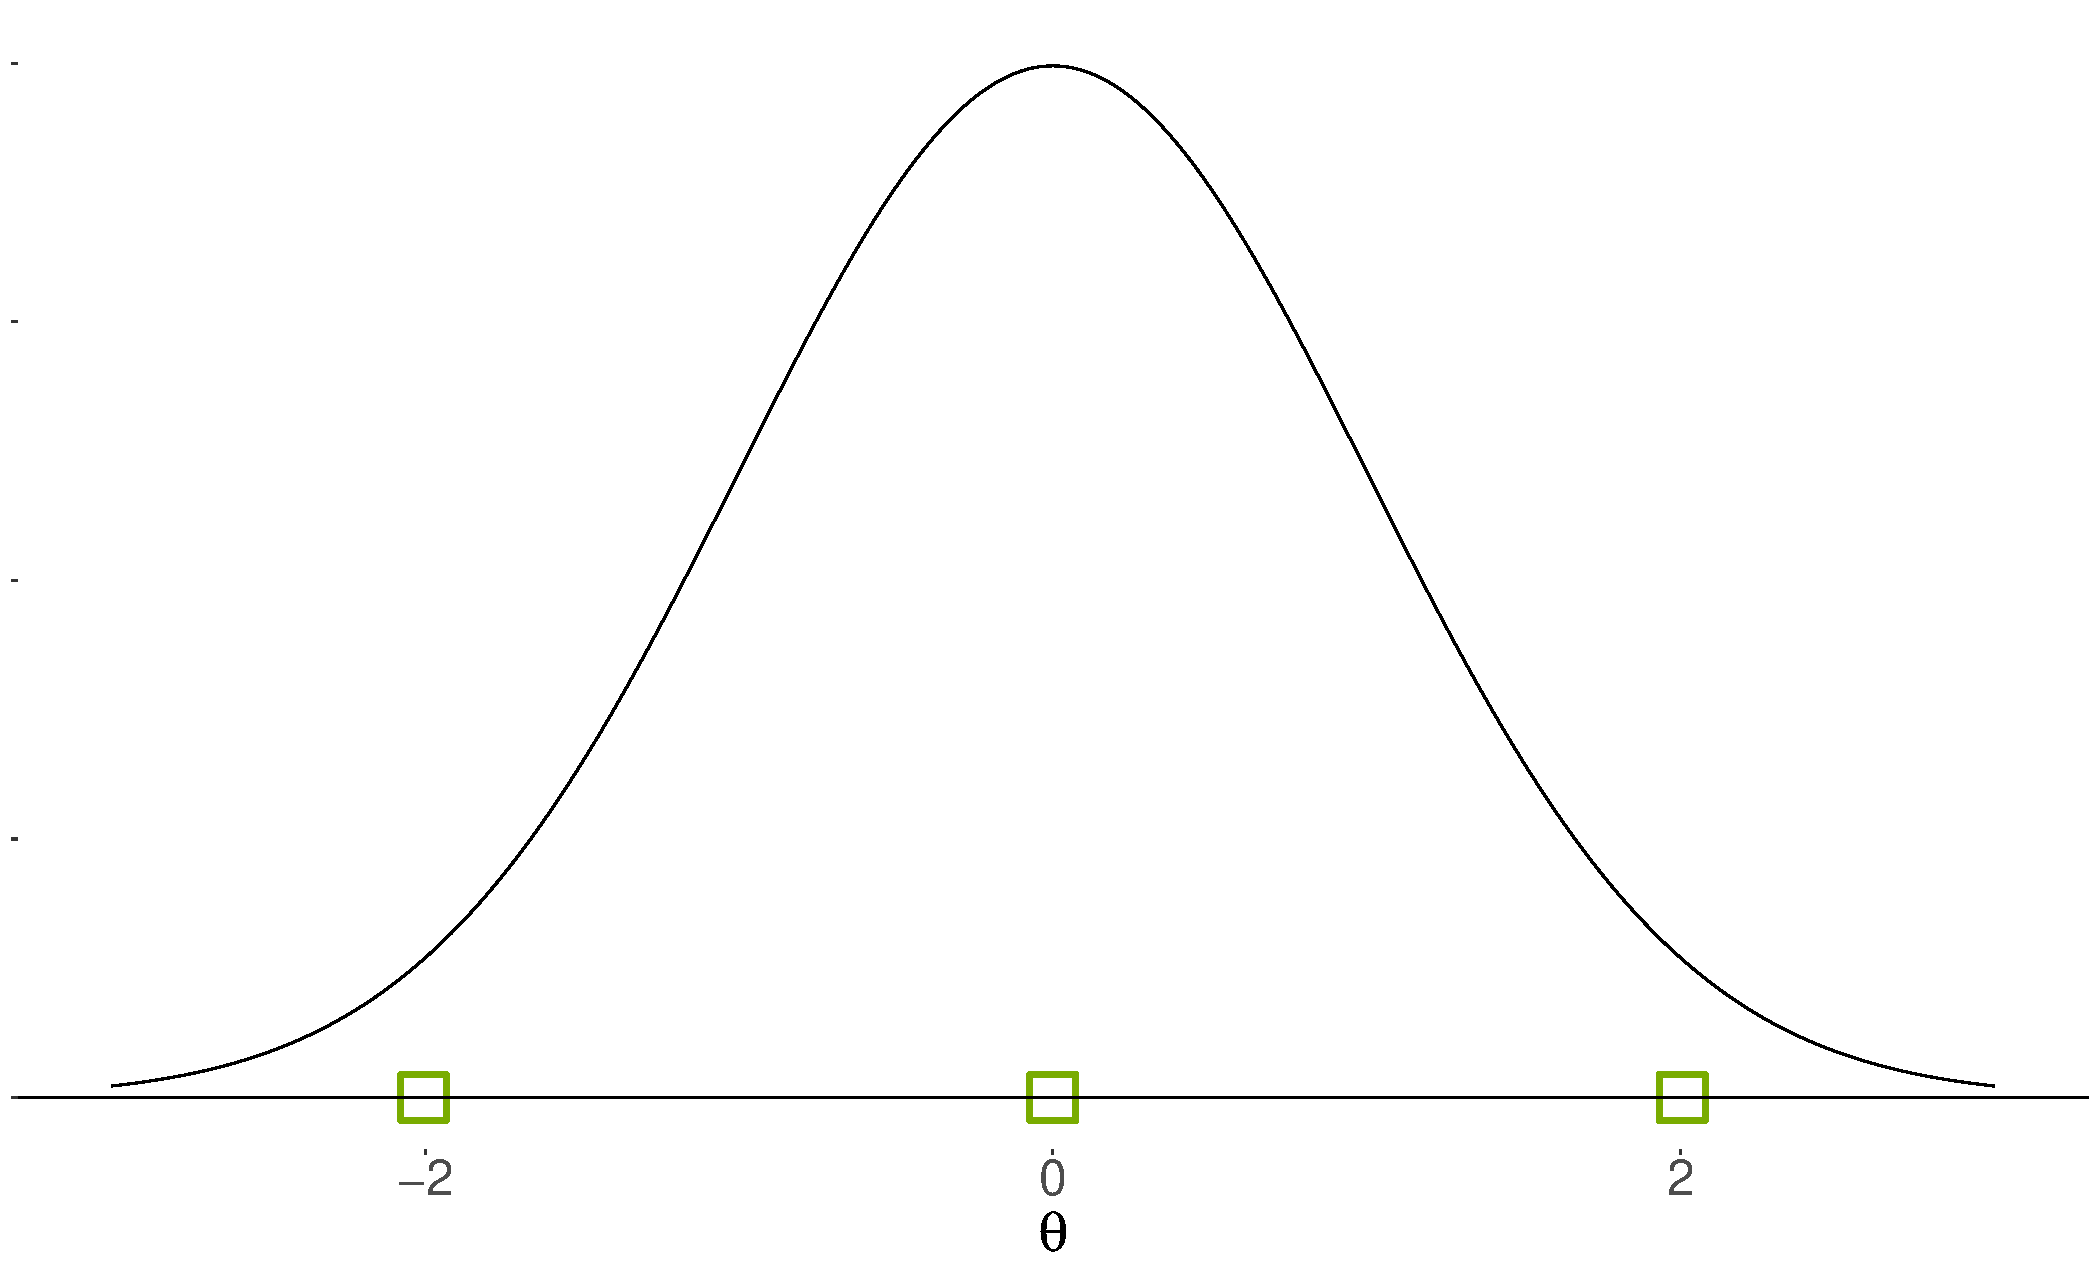
\includegraphics[width=.80\linewidth]{eip}
		\end{figure}
		\onslide<3>
		\begin{figure}
			\centering
			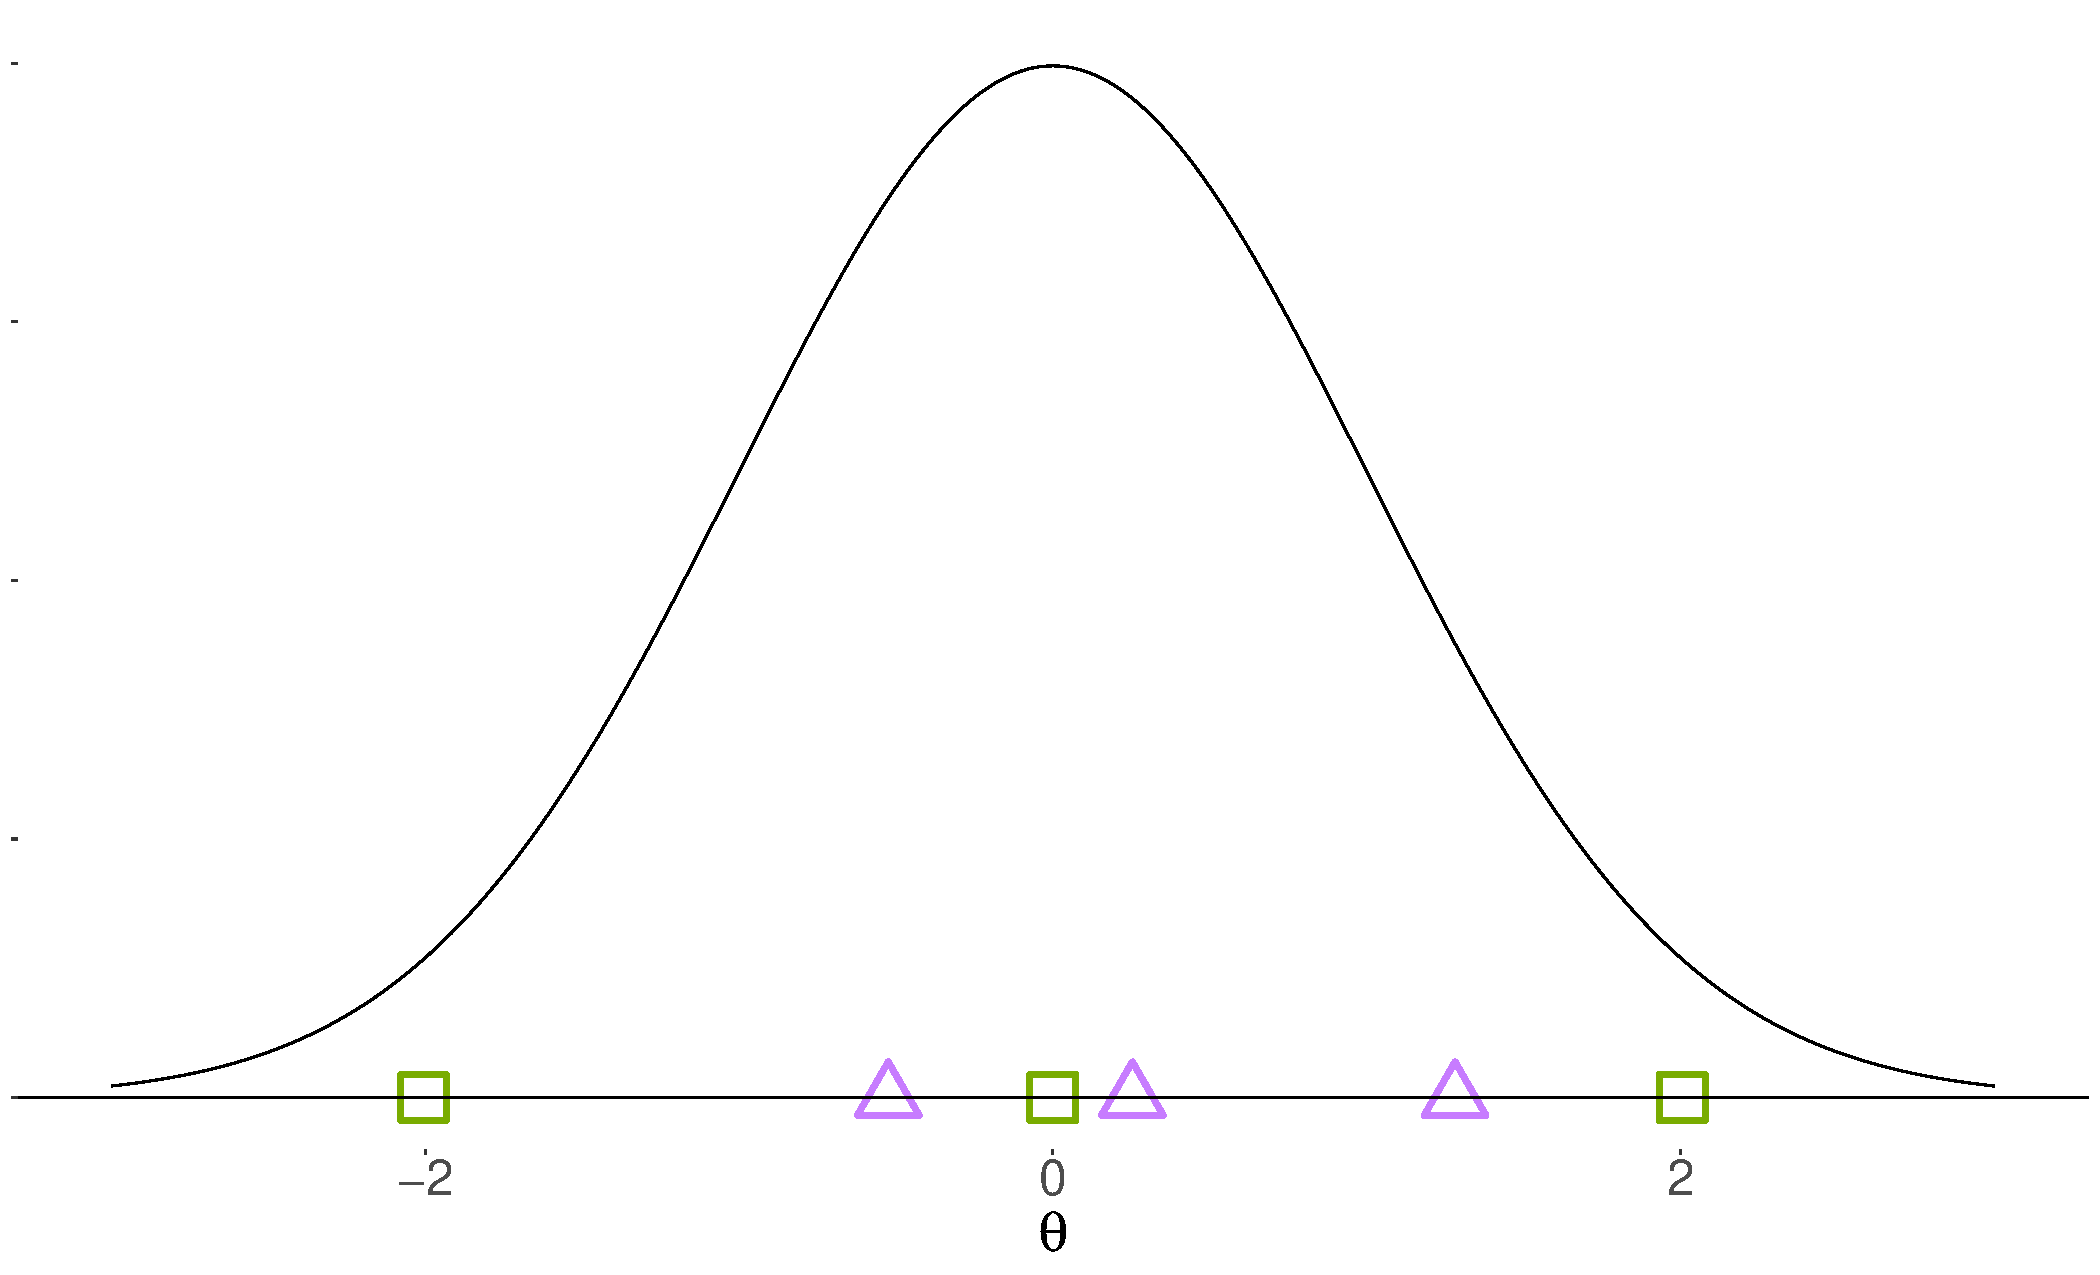
\includegraphics[width=.80\linewidth]{latent}
		\end{figure}
	\end{overprint}

\begin{columns}[T]
	\onslide<2->
	\begin{column}{.50\linewidth}
		\begin{center}
			\textcolor{eip}{Equal Intervals Procedure}\\
			\small Equal segmentation
		\end{center}
	\end{column}
\onslide<3->
	\begin{column}{.50\linewidth}
	\begin{center}
		\textcolor{uip}{Unequal Intervals Procedure}\\
		\small Clustering
	\end{center}
\end{column}
\end{columns}
	
\end{frame}


\section[Simulation]{Simulation study}

\begin{frame}
	Comparison between the item selection procedures: 
	\begin{itemize}
		\item \textbf{\textcolor{bp}{Benchmark procedure (BP)}}: The $N$ items with the highest \emph{IIF}s are selected from the full-length test
		\item \textbf{\textcolor{eip}{Equal Intervals Procedure (EIP)}}: The $N$ items that maximize the information for each $\theta'$ obtained by dividing the latent trait into equal intervals are selected
		\item \textbf{\textcolor{uip}{Unequal Intervals Procedure (UIP)}}:  The $N$ items that maximize the information for each $\theta'$ obtained by clustering the latent trait are selected 
		\item \textbf{\textcolor{rp}{Random Procedure (RP)}}: $N$ items are randomly selected from the full-length tests 
	\end{itemize}
\vspace{3mm}
10, 30, 50, 70, 90-item short test forms from a  100-item full-length test 

\end{frame}

\begin{frame}
		\begin{columns}[T]
		\begin{column}{.50\linewidth}
			\begin{center}
				1000 respondents $p$
			\end{center}
			\begin{enumerate}
				\item Normal distribution $p \sim \mathcal{N}(0,1)$
				\item Positive skewed distribution $p \sim Beta(1, 100)$ \tiny (linearly transformed to obtain negative values) 
				\item \normalsize Uniform distribution $p \sim \mathcal{U}(-3,3)$
			\end{enumerate}
			
		\end{column}
		
		\begin{column}{.50\linewidth}
			\begin{center}
				100 items $j$:
			\end{center}
			\begin{itemize}
				\item $b \sim \mathcal{U}(-3,3)$
				\item  $a \sim \mathcal{U}(0.40,2)$
			\end{itemize}
		\end{column}
	\end{columns}
\end{frame}


\begin{frame}{An overall look}
\begin{figure}
	\centering
	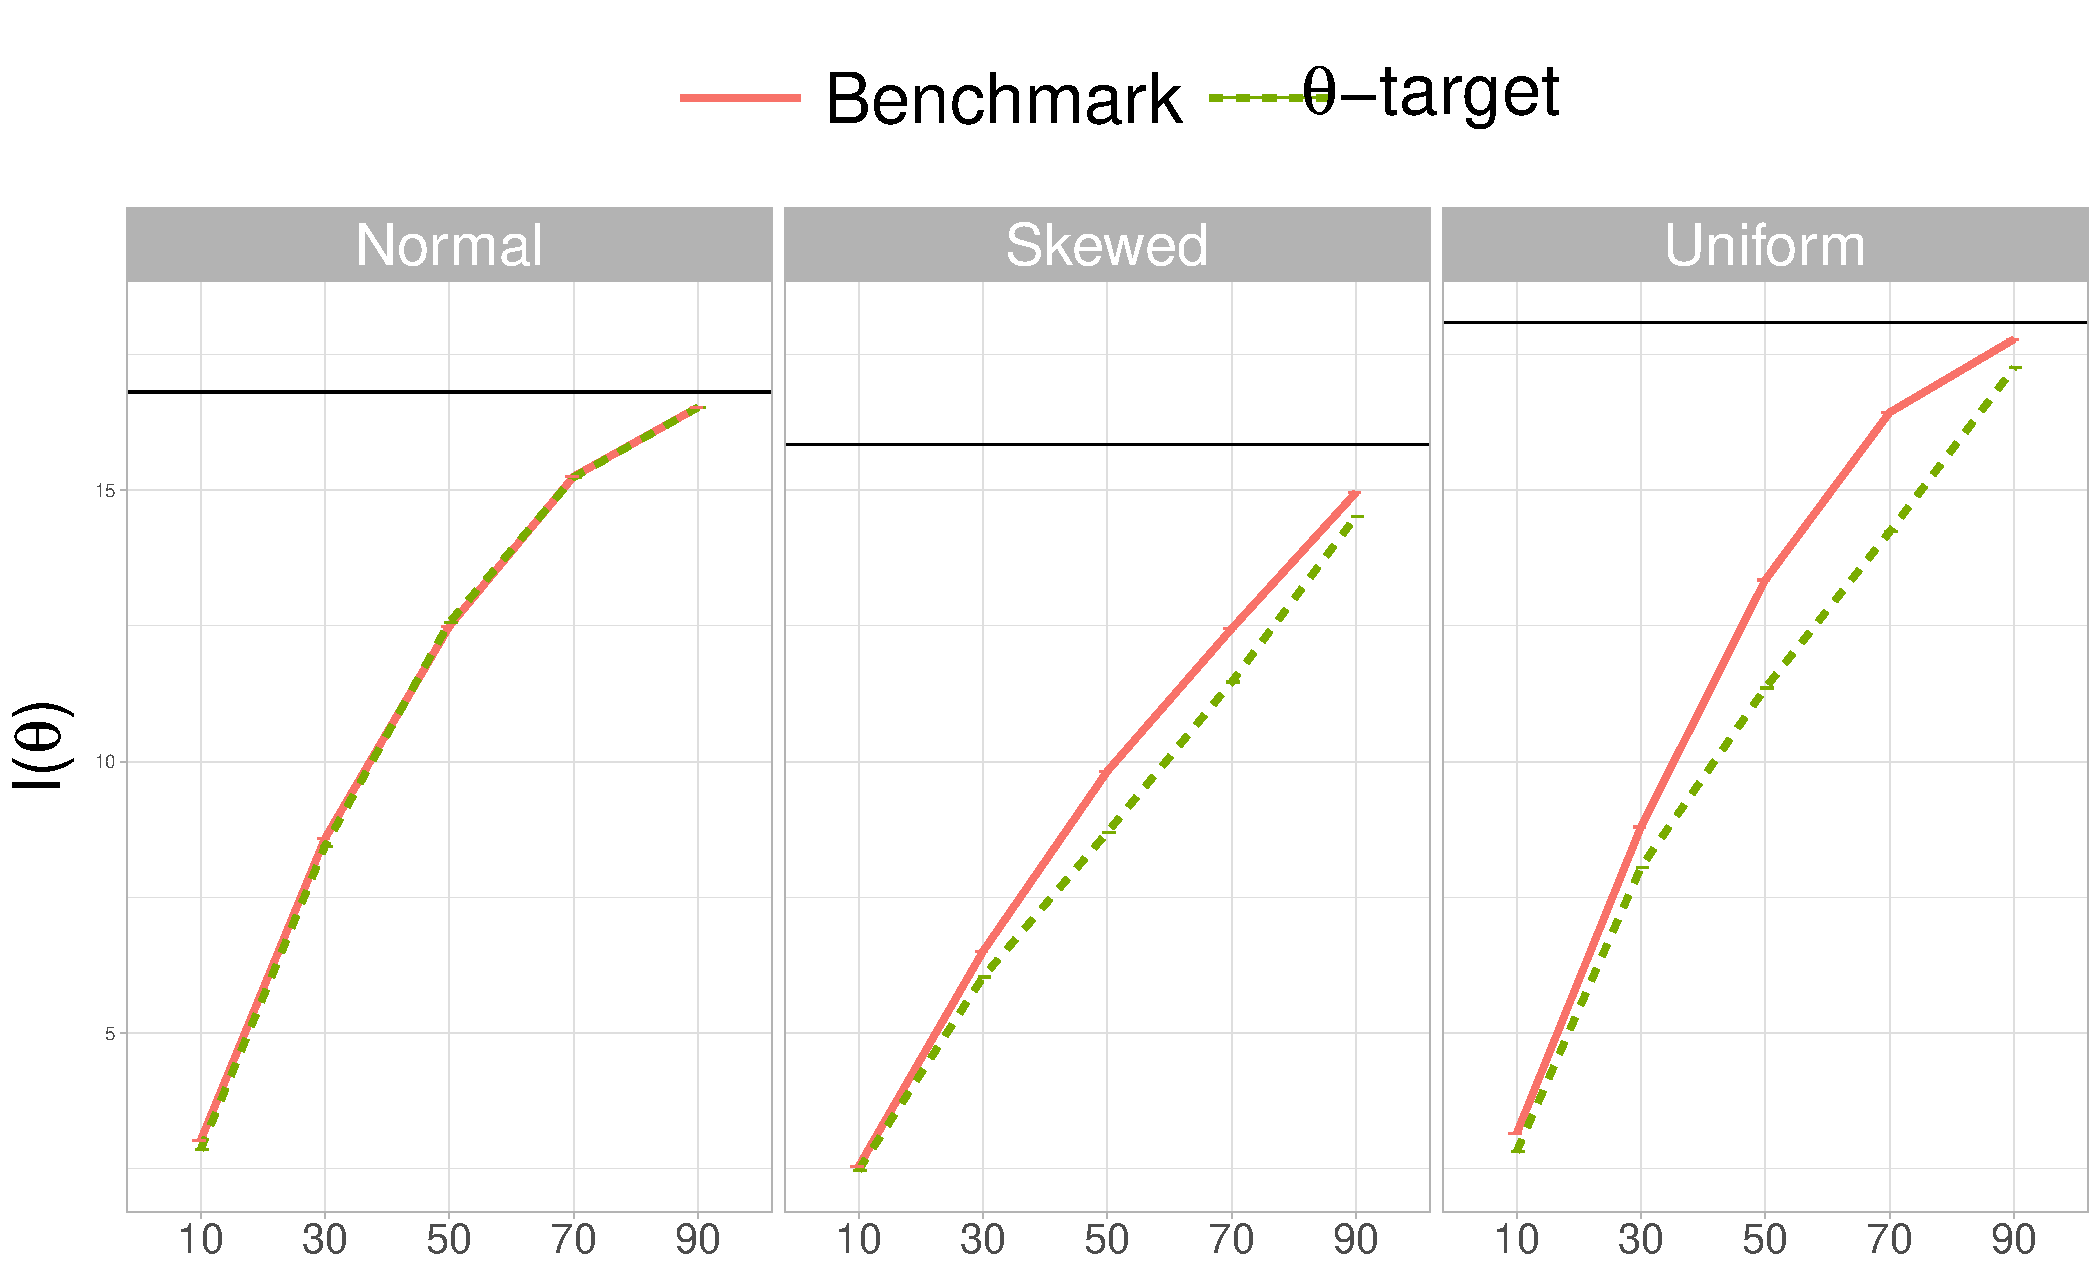
\includegraphics[width=.90\linewidth]{img/info.pdf}
	\caption{Overall Information of the short test forms}
\end{figure}
\end{frame}

\begin{frame}{A closer look}
	\begin{figure}
		\centering
		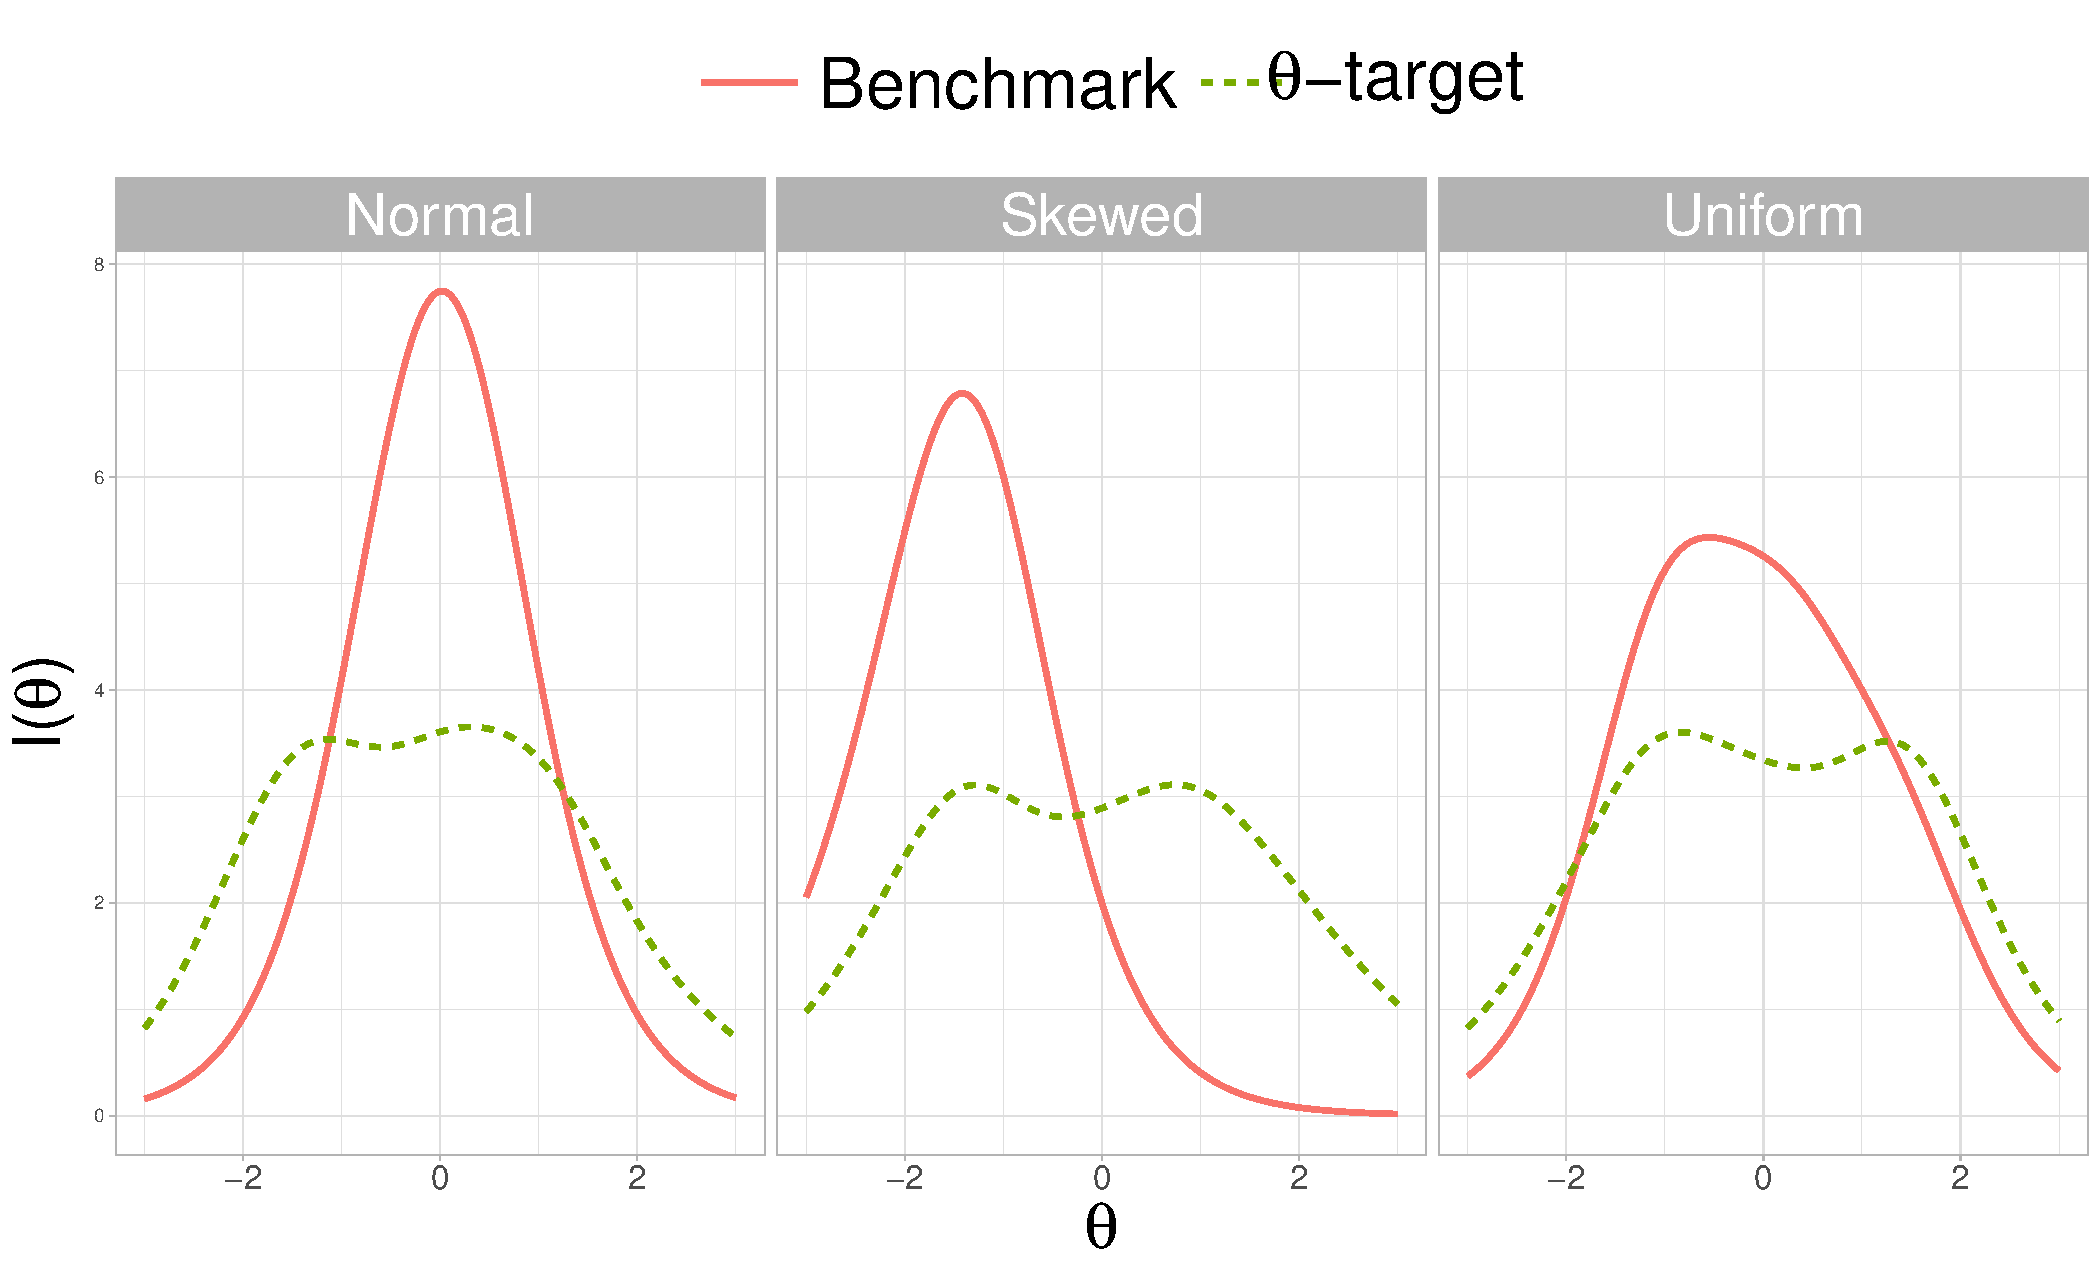
\includegraphics[width=.90\linewidth]{img/infoDetails.pdf}
		\caption{TIF of the 10-item short test form}
	\end{figure}
\end{frame}

\begin{frame}{An even closer look}
	\begin{figure}
		\centering
		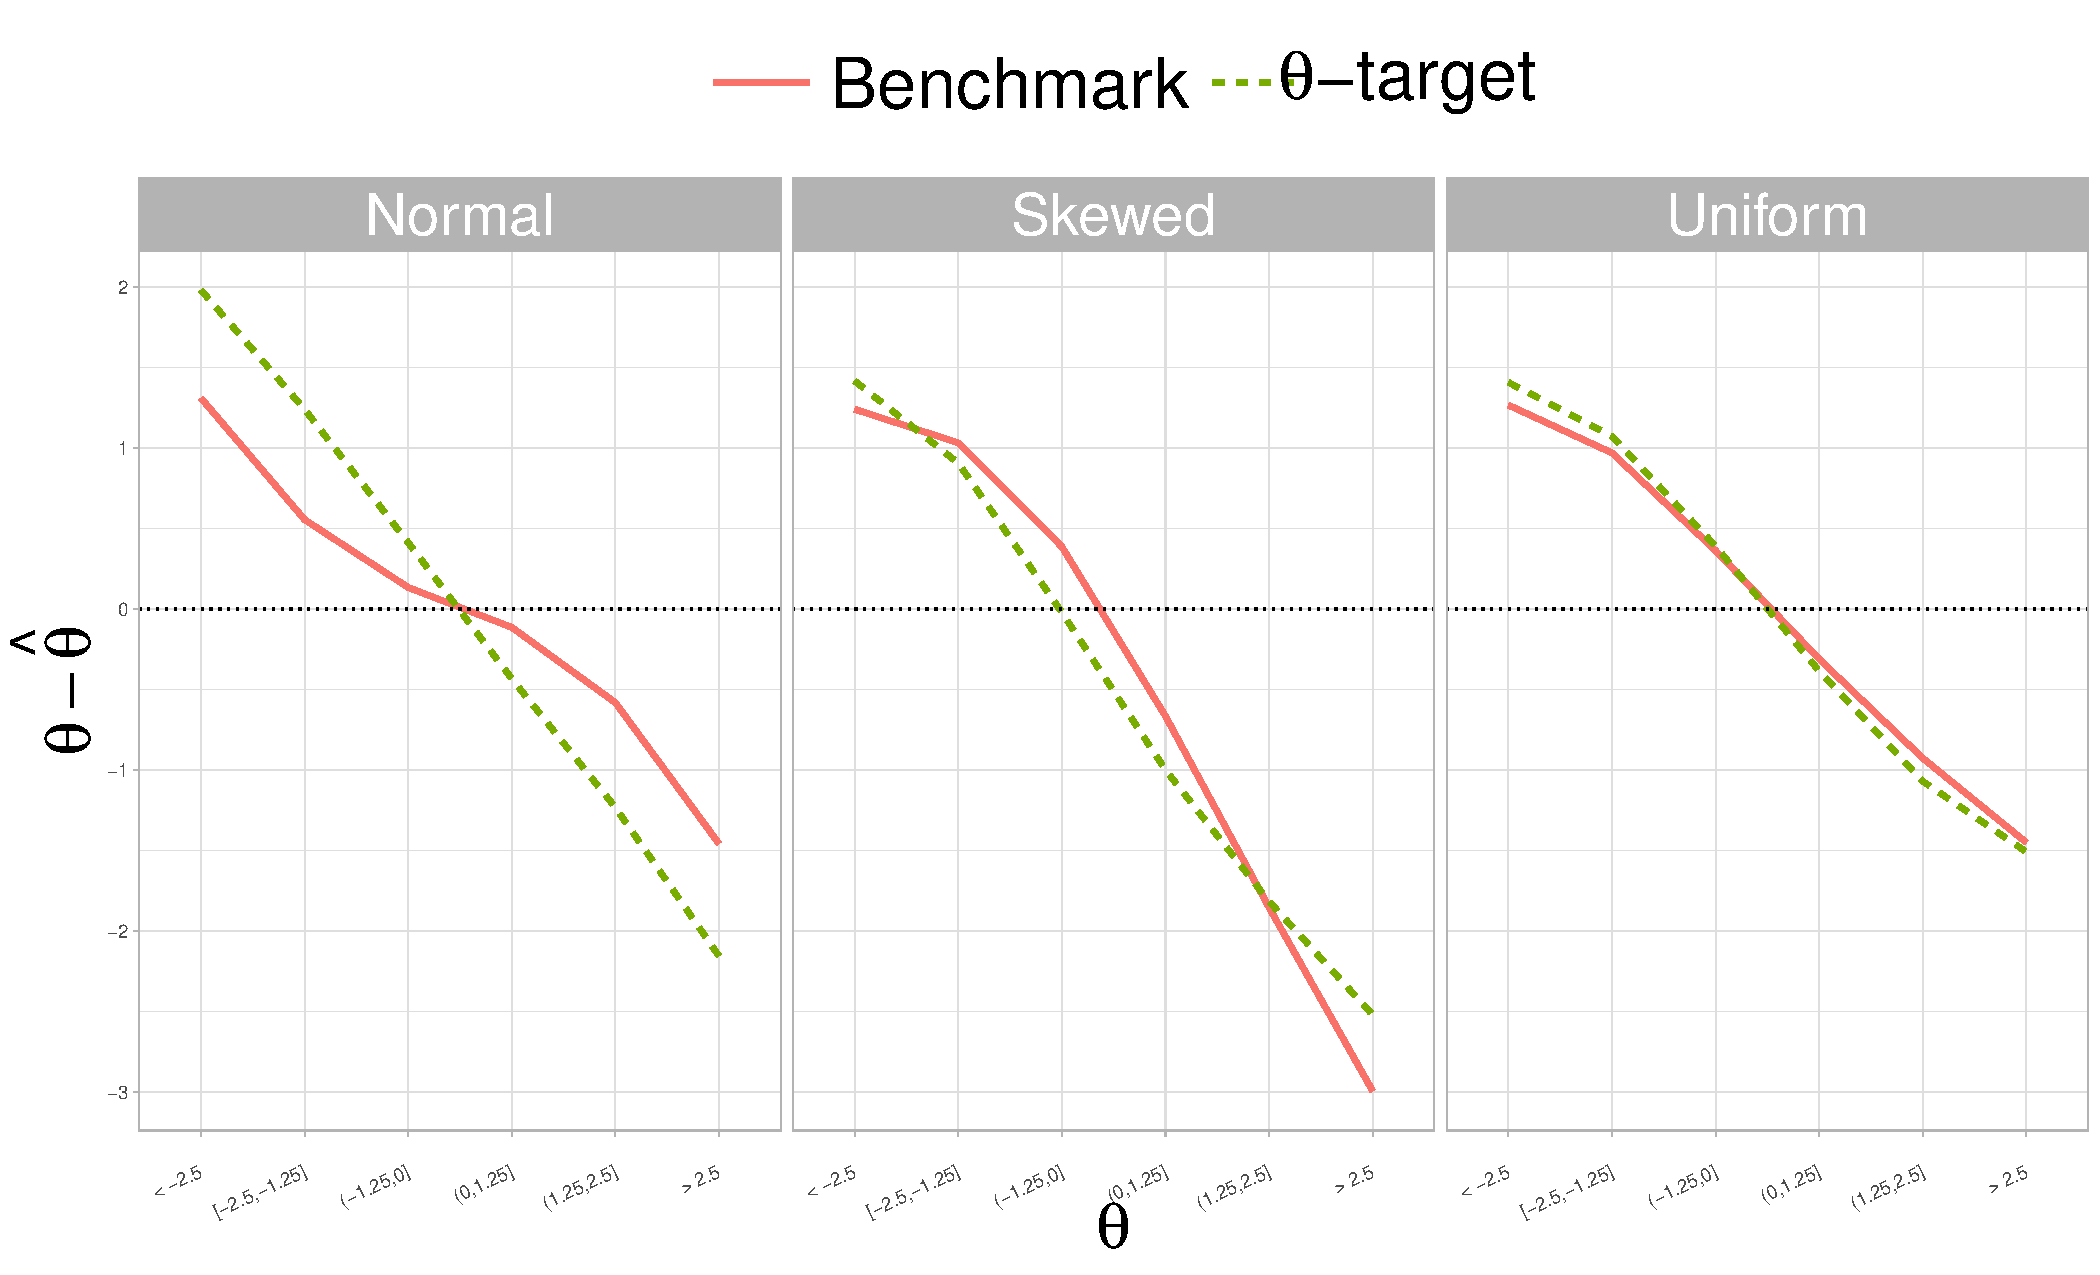
\includegraphics[width=.90\linewidth]{img/BIAS.pdf}
		\caption{$bias = \theta - \hat{\theta}$ of the 10-item short test form}
	\end{figure}
\end{frame}

\section[Final remarks]{Some final remarks}

\begin{frame}


\begin{exampleblock}{Good!}
	
	There's no ``one-fits-all'' solution
	
		\vspace{2mm}
		
		 The $\theta$ distribution is a key element
\end{exampleblock}

\pause
\begin{alertblock}{..but work is still needed}
		
				\vspace{2mm}
		Real life applications are missing
		
				\vspace{2mm}
		The CAT is missing
\end{alertblock}

\end{frame}

\begin{frame}[plain]
	\vspace{2cm}
	\begin{center}
		\large{Thank you!}
		
		\vspace{3mm}
		\texttt{ottavia.epifania@unipd.it}
		
	\begin{figure}
		\centering
		
\includegraphics[width=0.4\linewidth]{img/codeSlide}
	\end{figure}
	
	
	\end{center}
\end{frame}

\end{document}